%%%%%%%%%%%%%%%%%%%%%%%%%%%%%%%%%%%%%%%%%
% Beamer Presentation
% LaTeX Template
% Version 1.0 (10/11/12)
%
% This template has been downloaded from:
% http://www.LaTeXTemplates.com
%
% License:
% CC BY-NC-SA 3.0 (http://creativecommons.org/licenses/by-nc-sa/3.0/)
%
%%%%%%%%%%%%%%%%%%%%%%%%%%%%%%%%%%%%%%%%%

%----------------------------------------------------------------------------------------
%	PACKAGES AND THEMES
%----------------------------------------------------------------------------------------

\documentclass{beamer}

\mode<presentation> {

% The Beamer class comes with a number of default slide themes
% which change the colors and layouts of slides. Below this is a list
% of all the themes, uncomment each in turn to see what they look like.

%\usetheme{default}
%\usetheme{AnnArbor}
%\usetheme{Antibes}
%\usetheme{Bergen}
%\usetheme{Berkeley}
%\usetheme{Berlin}
%\usetheme{Boadilla}
%\usetheme{CambridgeUS}
%\usetheme{Copenhagen}
%\usetheme{Darmstadt}
%\usetheme{Dresden}
%\usetheme{Frankfurt}
%\usetheme{Goettingen}
%\usetheme{Hannover}
%\usetheme{Ilmenau}
%\usetheme{JuanLesPins}
%\usetheme{Luebeck}
\usetheme{Madrid}
%\usetheme{Malmoe}
%\usetheme{Marburg}
%\usetheme{Montpellier}
%\usetheme{PaloAlto}
%\usetheme{Pittsburgh}
%\usetheme{Rochester}
%\usetheme{Singapore}
%\usetheme{Szeged}
%\usetheme{Warsaw}

% As well as themes, the Beamer class has a number of color themes
% for any slide theme. Uncomment each of these in turn to see how it
% changes the colors of your current slide theme.

%\usecolortheme{albatross}
%\usecolortheme{beaver}
%\usecolortheme{beetle}
%\usecolortheme{crane}
%\usecolortheme{dolphin}
%\usecolortheme{dove}
%\usecolortheme{fly}
%\usecolortheme{lily}
%\usecolortheme{orchid}
%\usecolortheme{rose}
%\usecolortheme{seagull}
\usecolortheme{seahorse}
%\usecolortheme{whale}
%\usecolortheme{wolverine}

%\setbeamertemplate{footline} % To remove the footer line in all slides uncomment this line
%\setbeamertemplate{footline}[page number] % To replace the footer line in all slides with a simple slide count uncomment this line

%\setbeamertemplate{navigation symbols}{} % To remove the navigation symbols from the bottom of all slides uncomment this line
\setbeamertemplate{blocks}[rounded][shadow=false]
\setbeamertemplate{section in toc}{\inserttocsectionnumber.~\inserttocsection}


}

\usepackage{graphicx} % Allows including images
\usepackage{booktabs} % Allows the use of \toprule, \midrule and \bottomrule in tables


\usepackage{xcolor}
\usepackage{listings}

\definecolor{mGreen}{rgb}{0,0.5,0}
\definecolor{mGray}{rgb}{0.5,0.5,0.5}
\definecolor{mPurple}{rgb}{0.58,0,0.82}
\definecolor{backgroundColour}{rgb}{0.95,0.95,0.92}


\lstloadlanguages{{C}}

\lstdefinestyle{CStyle}{
   % backgroundcolor=\color{backgroundColour},   
    commentstyle=\color{mGreen},
    keywordstyle=\color{magenta},
    numberstyle=\tiny\color{mGray},
    stringstyle=\color{mPurple},
    basicstyle=\footnotesize,
    breakatwhitespace=false,         
    breaklines=true,                 
    captionpos=b,                    
    keepspaces=true,                 
    numbers=left,                    
    numbersep=5pt,                  
    showspaces=false,                
    showstringspaces=false,
    showtabs=false,                  
    tabsize=2,
    language=C,
    aboveskip=\smallskipamount,
    belowskip=\smallskipamount,
    mathescape=true,
    morekeywords = {assert},
    moredelim=**[is][\only<+>{\color{black}\lstset{style=highlight}}]{~}{~},
    literate= {|->}{{$\mapsto$}}1 {_L}{{$_L$}}1,
}

\lstdefinestyle{CStyleNoNum}{
   % backgroundcolor=\color{backgroundColour},   
    commentstyle=\color{mGreen},
    keywordstyle=\color{magenta},
    numberstyle=\tiny\color{mGray},
    stringstyle=\color{mPurple},
    basicstyle=\footnotesize,
    breakatwhitespace=false,         
    breaklines=true,                 
    captionpos=b,                    
    keepspaces=true,                 
    %numbers=left,                    
    %numbersep=5pt,                  
    showspaces=false,                
    showstringspaces=false,
    showtabs=false,                  
    tabsize=2,
    language=C,
    aboveskip=\smallskipamount,
    belowskip=\smallskipamount,
    mathescape=true,  
    morekeywords = {assert},
    moredelim=**[is][\only<+>{\color{black}\lstset{style=highlight}}]{~}{~},
    literate= {|->}{{$\mapsto$}}1 {_L}{{$_L$}}1,
}

\lstdefinestyle{highlight}{
  keywordstyle=\color{magenta},
  commentstyle=\color{mGreen},
}

\lstdefinestyle{CStyleOverlay}{
   % backgroundcolor=\color{backgroundColour}, 
    %basicstyle=\footnotesize,    
    basicstyle=\footnotesize\color{black!40},
  	keywordstyle=\color{black!40},%{red!40},
  	commentstyle=\color{black!40},%{green!40},  
    %commentstyle=\color{mGreen},
    %keywordstyle=\color{magenta},
    numberstyle=\tiny\color{mGray},
    stringstyle=\color{mPurple},
    breakatwhitespace=false,         
    breaklines=true,                 
    captionpos=b,                    
    keepspaces=true,                 
    numbers=left,                    
    numbersep=5pt,                  
    showspaces=false,                
    showstringspaces=false,
    showtabs=false,                  
    tabsize=2,
    language=C,
    aboveskip=\smallskipamount,
    belowskip=\smallskipamount,
    mathescape=true,
    morekeywords = {assert},
    moredelim=**[is][\only<+-+(1)>{\color{black}\lstset{style=highlight}}]{~}{~},
    moredelim=**[is][\only<.(1)>{\color{black}\lstset{style=highlight}}]{@@}{@@},
    moredelim=**[is][\only<6>{\color{black}\lstset{style=highlight}}]{£}{£},
    moredelim=**[is][\only<6>{\color{black}\lstset{style=highlight}}]{**}{**},
    literate= {|->}{{$\mapsto$}}1 {_L}{{$_L$}}1 {_(L-1)}{{$_{L-1}$}}3,
    escapeinside={µ}{µ},
    %moredelim=**[is][\only<+>{\color{red}}]{@@}{@@},
}
\let\origthelstnumber\thelstnumber
\makeatletter
\newcommand*\Suppressnumber{%
  \lst@AddToHook{OnNewLine}{%
    \let\thelstnumber\relax%
     \advance\c@lstnumber-\@ne\relax%
    }%
}
\newcommand*\Reactivatenumber[1]{%
  \setcounter{lstnumber}{\numexpr#1-1\relax}
  \lst@AddToHook{OnNewLine}{%
   \let\thelstnumber\origthelstnumber%
   \refstepcounter{lstnumber}
  }%
}

\makeatother
\usepackage{tikz}


\usepackage{amsmath}
\usepackage{amssymb}
\usepackage[inference]{semantic}
\usepackage{xargs}
\usepackage{etoolbox}

\makeatletter
\def\@myenvname{equation}
\newcommand{\eqIfNoEq}[1]{%
  \ifx\@currenvir\@myenvname
    #1
  \else
    \begin{equation}#1
    \end{equation}
  \fi}
\newcommand{\eqIfNoMM}[1]{%
  \ifmmode
    #1
  \else
    \begin{equation}#1
    \end{equation}
  \fi}
\makeatother

\let\oldinference\inference
%\renewcommand{\inference}[2]{\[\oldinference{#1}{#2}\]}
\renewcommandx*\inference[3][3]{
\ifstrempty{#3}{
\eqIfNoEq{\oldinference{#1}{#2}}
}{
\eqIfNoEq{\oldinference{#1}{#2\tagsc{#3}}}
}
}

\newbool{shouldUseCompile}
\setbool{shouldUseCompile}{true}
\newcommandx*\triple[7][2,3,6,7]{\{#1\}^{#2}_{#3}\ #4\ \{#5\}^{#6}_{#7}} %\ifmmode to enforce math mode, but this should work without the checks
\newcommandx*\compile[3][3]{\ifbool{shouldUseCompile}{#1 \leadsto_{#3} #2}{#1}}

\usepackage{enumitem}
\setitemize{label=\usebeamerfont*{itemize item}%
  \usebeamercolor[fg]{itemize item}
  \usebeamertemplate{itemize item}}

\newcommandx*\simrelcom[2]{
{#1} \ R\ {#2}
}
\newcommandx*\backtranslation[1]{\langle\langle #1 \rangle\rangle}



%blue boxes
\definecolor{myblue}{rgb}{.84, .84, .95}
\usepackage{empheq}
\setbeamercolor{block body}{bg=myblue}


\newlength\mytemplen
\newsavebox\mytempbox

\makeatletter
\newcommand\mybluebox{%
    \@ifnextchar[%]
       {\@mybluebox}%
       {\@mybluebox[0pt]}}

\def\@mybluebox[#1]{%
    \@ifnextchar[%]
       {\@@mybluebox[#1]}%
       {\@@mybluebox[#1][0pt]}}

\def\@@mybluebox[#1][#2]#3{
    \sbox\mytempbox{#3}%
    \mytemplen\ht\mytempbox
    \advance\mytemplen #1\relax
    \ht\mytempbox\mytemplen
    \mytemplen\dp\mytempbox
    \advance\mytemplen #2\relax
    \dp\mytempbox\mytemplen
    \colorbox{myblue}{\hspace{1em}\usebox{\mytempbox}\hspace{1em}}}

\makeatother

%gets rid of footer
%will override 'frame number' instruction above
%comment out to revert to previous/default definitions
\setbeamertemplate{footline}{}
%gets rid of bottom navigation symbols
\setbeamertemplate{navigation symbols}{}

%Gannt chart stuff:
\usepackage{pgfgantt}
\usepackage{xparse}
\usepackage{enumitem}% http://ctan.org/pkg/enumitem

\NewDocumentCommand\textganttbar{O{} O{} mmmm}{%
    \ganttbar[#1,bar/.append style={alias=tmp}]{#3}{#5}{#6}
    \node [font=\footnotesize,at={(tmp)},#2]  {#4};
}

\tikzset{
  above bar/.style={
    at={(tmp.north)},anchor=south
    },
  below bar/.style={
    at={(tmp.south)},anchor=north
    }
}


%----------------------------------------------------------------------------------------
%	TITLE PAGE
%----------------------------------------------------------------------------------------

\title[Linear Capability Verification]{Linear capabilities for fully abstract
compilation of separation-logic-verified code} % The short title appears at the bottom of every slide, the full title is only on the title page

\author[Thomas Van Strydonck]{\underline{Thomas Van Strydonck} \and Dominique Devriese \and Frank Piessens} % Your name
\institute[KU Leuven] % Your institution as it will appear on the bottom of every slide, may be shorthand to save space
{
KU Leuven \\ % Your institution for the title page
\medskip
\textit{thomas.vanstrydonck@cs.kuleuven.be} % Your email address
}
\date{\today} % Date, can be changed to a custom date

\begin{document}

%Showing off the current section
\AtBeginSection[]{
  \begin{frame}{Outline}
  \small \tableofcontents[currentsection, hideothersubsections]
  \end{frame} 
}

%%Start of the presentation

\begin{frame}
\titlepage % Print the title page as the first slide 
\end{frame}

\begin{frame}
\frametitle{Problem: Preserving verification during compilation}

\begin{columns}
\begin{column}{0.65\textwidth}
\begin{itemize}
\item Separation logic in verification tools
	\begin{itemize}
	\item Sound
	\item Modular
	\end{itemize}
\item \textbf{Problem}: Guarantees \emph{lost} in untrusted context %why? keeping references etc; multithreading,...
\item \textbf{Solution}: Compiler enforces separation logic contracts  %compiles vf -> uvf
\end{itemize}
\end{column}
\begin{column}{0.37\textwidth}
\def\firstcircle{(0,0) circle (2cm)}
\def\secondcircle{(0,0) circle (1.3cm)}
\colorlet{circle edge}{black!100}
\colorlet{circle area}{black!0}
\tikzset{filled/.style={fill=circle area, draw=circle edge, thick}, outline/.style={draw=circle edge, thick}}

%\setlength{\parskip}{5mm}
\begin{tikzpicture}
    \draw[outline] \firstcircle node {Verified Cmpnt};
    \draw[outline] \secondcircle node {};
    \node at (0,-1.6) (nodeA) {Context};
\end{tikzpicture}
\end{column}
\end{columns}
\end{frame}

%------------------------------------------------

\begin{frame}
\frametitle{The compiler}
\begin{columns}
\begin{column}{0.45\textwidth}
	\begin{block}{Source language}
	\begin{itemize}
	\item Regular verified C code
	\item \emph{Separation logic} annotated
		\begin{itemize}
		\item e.g. VeriFast syntax for concreteness
		\end{itemize}
	\end{itemize}
	\end{block}
\end{column}
\begin{column}{0.08\textwidth}
	\begin{figure}
	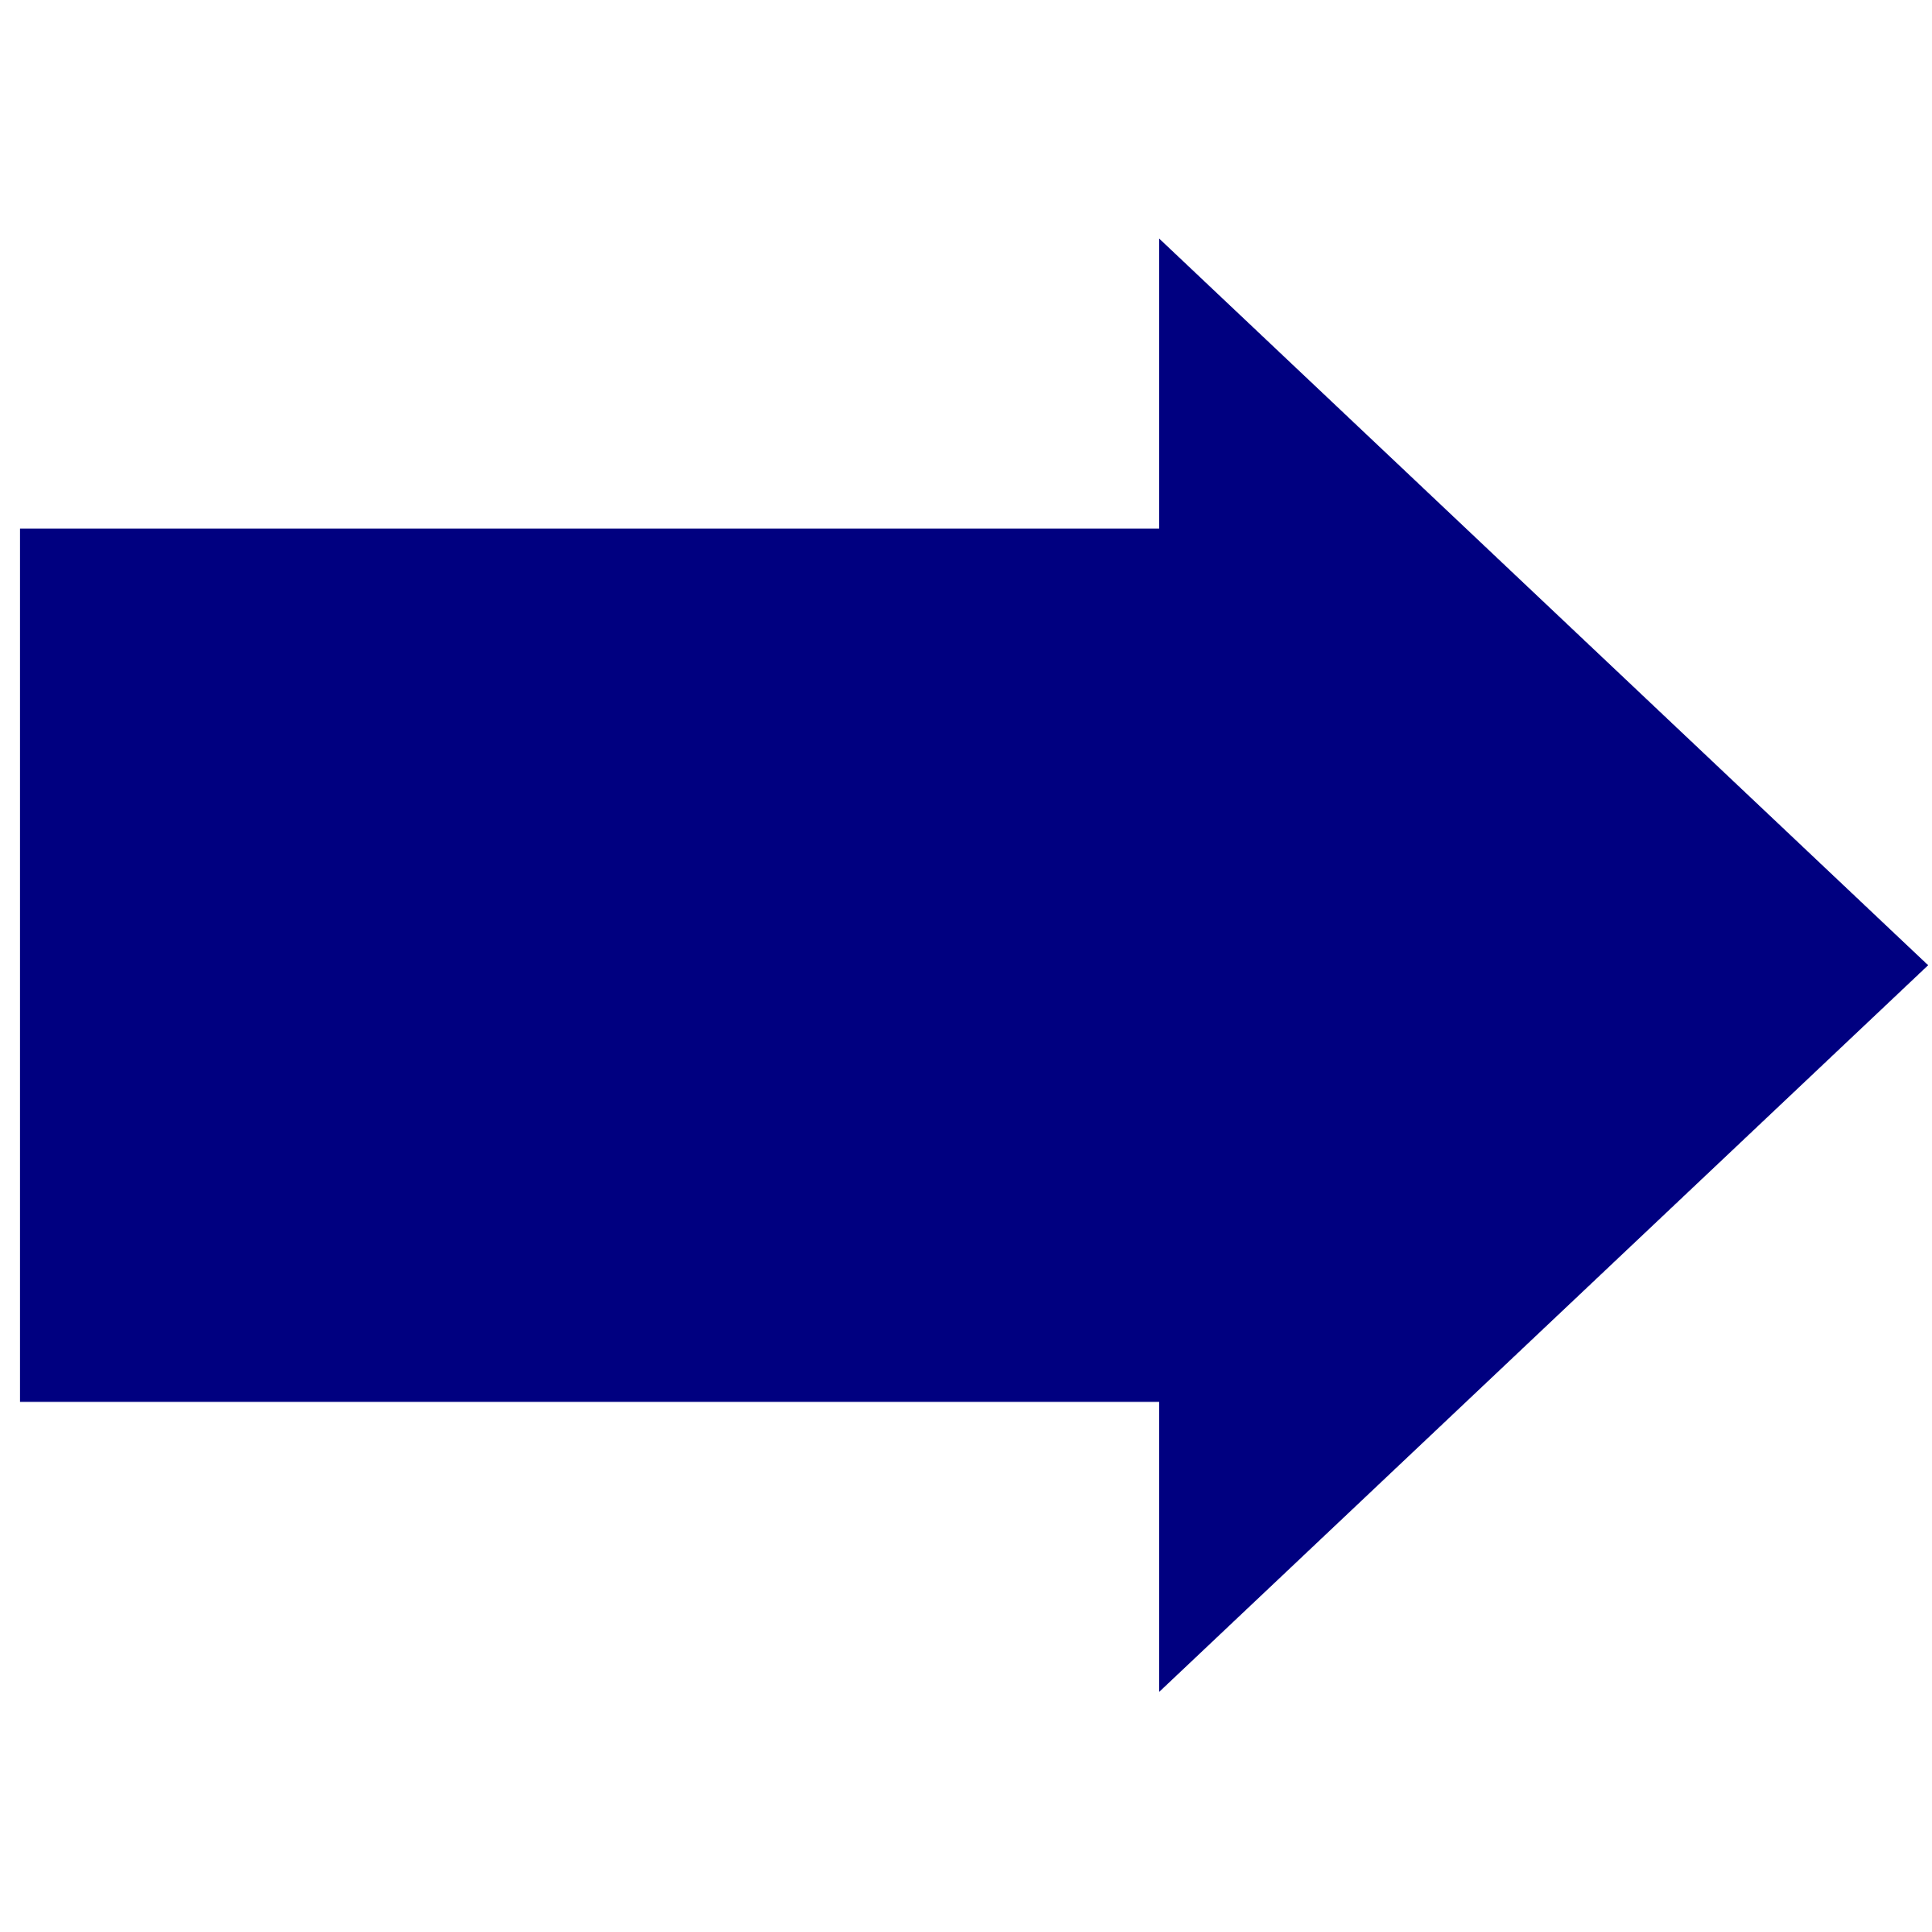
\includegraphics[width=0.8\linewidth]{BlueArrow}
	\end{figure}
\end{column}
\begin{column}{0.45\textwidth}
    \begin{block}{Target language}
	\begin{itemize}
	\item Regular unverified C code
	\item Support for \emph{capabilities} \\
		\begin{itemize}
		\item CHERI-inspired 
		\item Linear capabilities
		%\item Sealed capabilities %Q? Do we still need these? e.g. nested arrays wont contain nested capabilities; the nesting of capabilities was only a problem wiht AP's
		\end{itemize}
	\end{itemize}
	\end{block}
\end{column}
\end{columns}
%\vspace{1em}
\center No assembly hassle in C, but still unsafe (powerful attacker).

 %compiles vf -> uvf
\end{frame}

\begin{frame}
\frametitle{Overview} % Table of contents slide, comment this block out to remove it
\tableofcontents % Throughout your presentation, if you choose to use \section{} and \subsection{} commands, these will automatically be printed on this slide as an overview of your presentation
\end{frame}

\section{Problem context}

\begin{frame}[plain,c]
%\frametitle{A first slide}

\begin{center}
\Huge Linear capabilities for\\  fully abstract
compilation of \textbf{\underline{separation-logic-verified}} code
\end{center}
\end{frame}


\begin{frame}[fragile]
\frametitle{Separation Logic} 
\begin{itemize}
\item Substructural logic (linear aspects)
\item Program verification
\begin{itemize}
\item Sound %proof implies correct
\item Modular %per-module proofs
\end{itemize}
\item Contract-based, eg. :\\
\begin{columns}%<0>
\begin{column}{0.55\textwidth}
\begin{lstlisting}[style=CStylenoNum, captionpos = t, xleftmargin = 4em]
void p(int x,int *data)
//@pre data |-> _ * x > 0;
//@post data |-> x;
{*data = x}
\end{lstlisting}
\end{column}
\begin{column}{0.45\textwidth}
Notation:
\begin{itemize}
\item $\textcolor{mGreen}{\ast}$, $\textcolor{mGreen}{\mapsto}$ (chunk: permission)
\item @pre/post: contract\\
	\quad Consume/produce
\item Other annotations
\end{itemize}
\end{column}
\end{columns}
\vspace{1em}
\item Hoare-logic-style program proofs: $\Rightarrow \triple{P}{c}{Q}$\\
	\quad Functions: $\triple{@pre}{BODY}{@post}$
\end{itemize}
\end{frame}

\begin{frame}[plain,c]
%\frametitle{A first slide}

\begin{center}
\Huge \underline{\textbf{Linear capabilities}} for\\  fully abstract
compilation of separation-logic-verified code
\end{center}

\end{frame}


%------------------------------------------------

\begin{frame}
\frametitle{(Linear) Capabilities}

\begin{columns}
\begin{column}{0.5\textwidth}
	\textbf{Capability}: %Q? leave this out/reduce to one line? Or add figure? + source for figure?
\begin{itemize}
\item Unforgeable memory pointer
\item Grants permissions on memory region
\item Fine-grained memory protection
\item Capability machines (ex CHERI)
\end{itemize}
\end{column}
\begin{column}{0.5\textwidth}
\begin{figure}
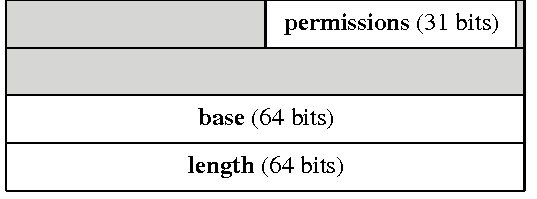
\includegraphics[width=\linewidth]{Capability}%Q? Reference? https://www.semanticscholar.org/paper/The-CHERI-capability-model-Revisiting-RISC-in-an-a-Woodruff-Watson/0657eb7e069c2c2c7cae6636704e0f7fb3bcd9fc
\end{figure}
\end{column}
\end{columns}
\vspace{.5em}

 %compiles vf -> uvf
%\textbf{Sealed Capability}: %Q? Delete
%Unaccessible until unsealed using an appropriate seal.
%\vspace{.5em}

\textbf{Linear Capability}: %Fits very well with consuming and producing in separation logic = linear aspects of separation logic
\begin{itemize}
\item Linearity = one-use! cfr e.g. Linear Logic
\item Non-copyable
$\Rightarrow$ callers/callees cannot keep copies
\item Intuitive: separation logic is linear
\end{itemize}
\end{frame}

%------------------------------------------------


\begin{frame}[plain,c]
%\frametitle{A first slide}
\begin{center}
\Huge Linear capabilities for\\  \textbf{\underline{fully abstract}}
compilation of separation-logic-verified code
\end{center}
\end{frame}

\begin{frame}
\frametitle{Full abstraction is sufficient} %Mention secure compilation?
 \setbeamercovered{transparent}
\begin{block}{Intuition}<1>
"Attacking the compiled code is as hard as attacking the source code" \\[1em]%Even though the target language is usually lower level and hence more powerful as an attacker
Fully abstract compiler $\Rightarrow$ compiled code upholds contracts\\
\end{block}
\only<2>{
\begin{block}{Definition of FA} %Q? or is this too trivial? It was a confusing bit for me at the start
= reflection and preservation of contextual equivalence $\simeq_{ctx}$ \\
\vspace{-1em}
\begin{align*}&s\simeq_{ctx}s' \Leftrightarrow [[s]]\simeq_{ctx}[[s']]\\
&\text{where } x\simeq_{ctx}x'\equiv \forall C: C[x]\Downarrow\ \Leftrightarrow C[x']\Downarrow
\end{align*}
$\supseteq$ preservation of integrity and confidentiality \\
\end{block}
} 
 %compiles vf -> uvf
\end{frame}

%------------------------------------------------

\begin{frame}
\frametitle{Goal: proving that contracts are compiled away safely by proving full abstraction}
 %\setbeamercovered{transparent}
\begin{columns}%<0>
\begin{column}{0.45\textwidth}
	\begin{block}{Source language}
	\begin{itemize}
	\item Regular verified C code
	\item \emph{Separation logic} annotated
		\begin{itemize}
		\item e.g. VeriFast syntax for concreteness
		\end{itemize}
	\end{itemize}
	\end{block}
\end{column}
\begin{column}{0.08\textwidth}
	\begin{figure}
	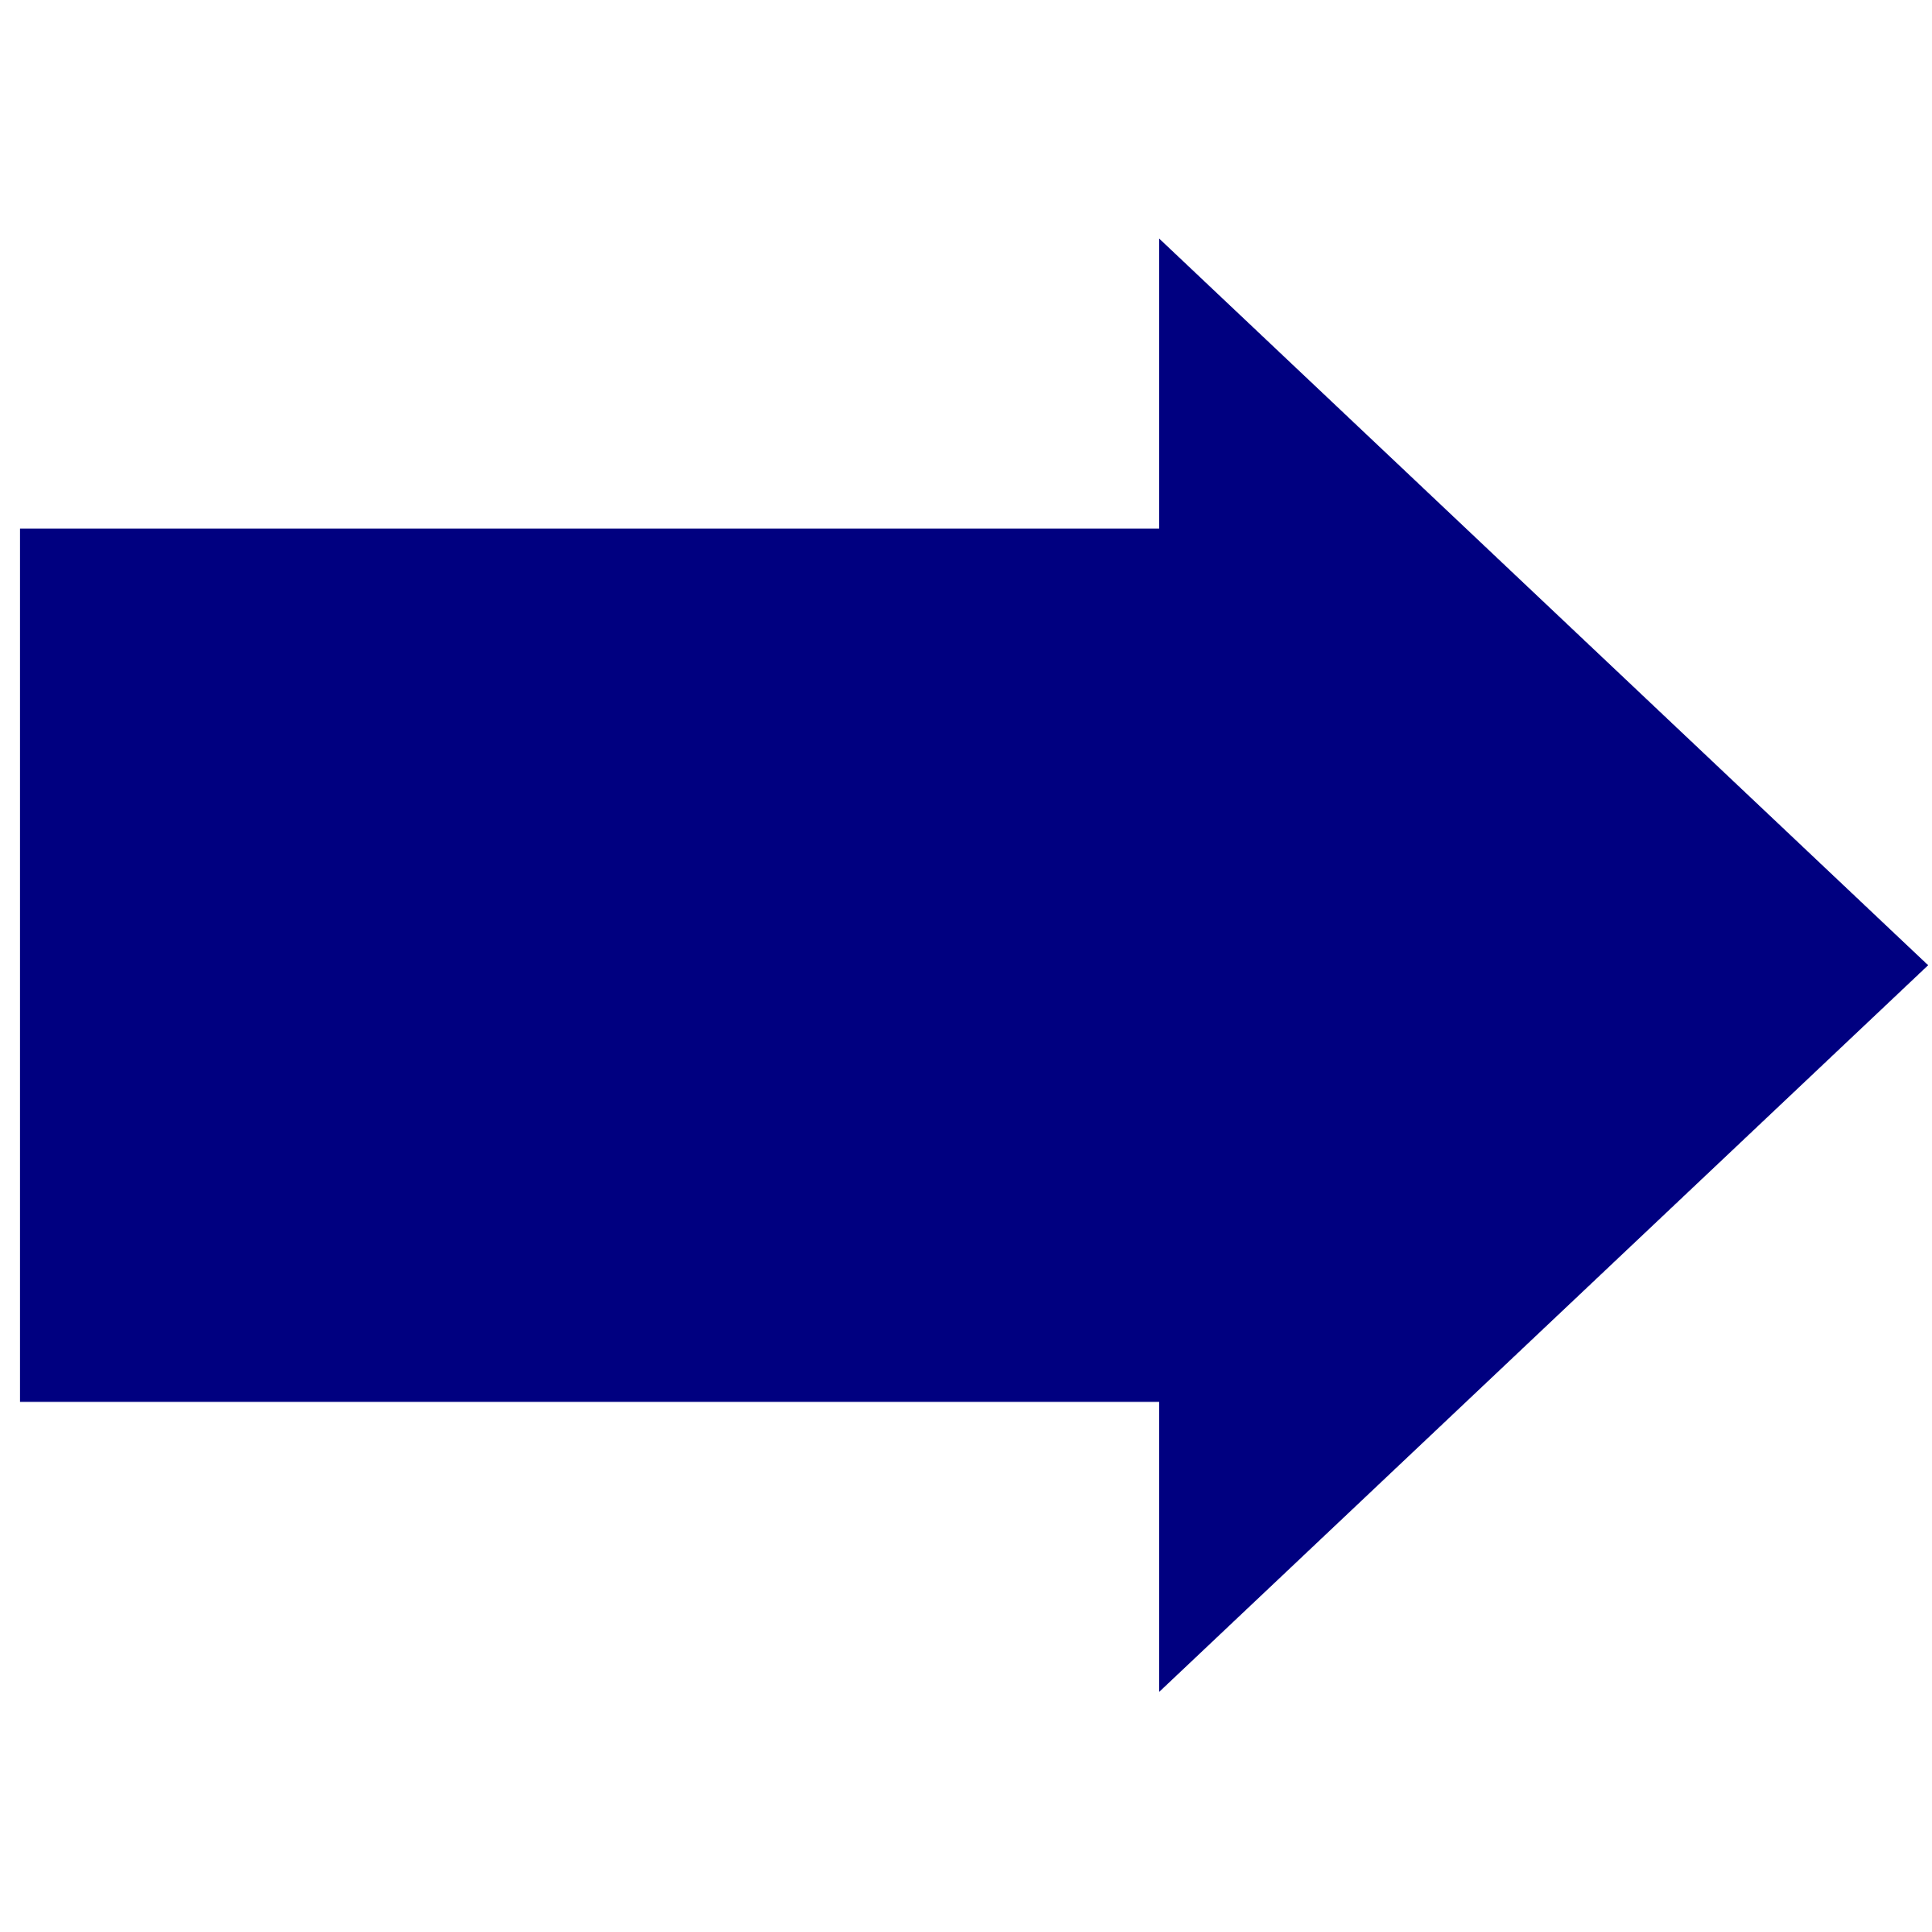
\includegraphics[width=0.8\linewidth]{BlueArrow}
	\end{figure}\vspace{-2em}
	\center \textbf{FA!}
\end{column}
\begin{column}{0.45\textwidth}
    \begin{block}{Target language}
	\begin{itemize}
	\item Regular unverified C code
	\item Support for \emph{capabilities}\\
		\begin{itemize}
		\item CHERI-inspired 
		\item Linear capabilities
		%\item Sealed capabilities %Q? Do we still need these? e.g. nested arrays wont contain nested capabilities; the nesting of capabilities was only a problem wiht AP's
		\end{itemize}
	\end{itemize}
	\end{block}
\end{column}
\end{columns}
\vspace{1em}
\textbf{Related work (Agten et al.)} %Q? maybe leave out? This is super relevant though, and underscores the advantage of fine-grainedness of capabilities wrt PMAs, but not everyone might know this
\begin{itemize}
\item Different hardware primitives\\%PMA's instead of capabilities\\
	$\Rightarrow$ Less fine-grained
\item Integrity, \emph{not} confidentiality

\end{itemize}
\end{frame}

%------------------------------------------------
\section{Compilation by example}

\begin{frame}[fragile]
\frametitle{Example program} %Q? zie code: afwijken van C - syntax; eerder in slides ook C-like schrijven? (anders ga je te veel moeten focussen op het low-level verschil tussen een pointer en een reference denk ik)
Illustrates approach\\
Based on \emph{separation logic derivation} (next slide)
\begin{columns}
\begin{column}{0.015\textwidth}
\end{column}
\begin{column}{0.55\textwidth}
\begin{figure}[h]
  \centering
\begin{lstlisting}[style=CStyle, captionpos = t]
void array_map(int n[], int *data, int L)
//@pre n |-> [_]_L * data |-> _;
//@post n |-> [_]_L * data |-> _;
{
	if (L == 0) { 
		skip;
	} else {
		//@split n[0];
		int newVal = p(n[0], data);
		n[0] = newVal;
		array_map(n+1, data, L-1);
		//@join n (n+1);
	}
	return; 
}
\end{lstlisting}
\end{figure}
\end{column}
\begin{column}{0.43\textwidth}
\begin{lstlisting}[style=CStyle, captionpos = t]
int p(int x, int *data)
//@pre data $\textcolor{mGreen}{\mapsto}$ _; 
//@post data $\textcolor{mGreen}{\mapsto}$ _;
{$\ldots$}
\end{lstlisting}
\begin{block}{Elements}
\begin{itemize}
\item array chunk notation: [$\cdot$]
\item @split/join: manipulate array chunks
\end{itemize}
\end{block}
\end{column}
\begin{column}{0.005\textwidth}
\end{column}
\end{columns}
\end{frame}
%------------------------------------------------
\begin{frame}
\frametitle{Separation logic derivation}
= proof of function contract\\
%= tree of Hoare triples related by separation logic axioms (e.g. \textsc{If}, \textsc{F-App}, $\ldots$)\\%Q? maybe show one step
\vspace{.5em}
%\textbf{Root} = the Hoare triple: $\{pre\}\ BODY\ \{post\}$\\
\vspace{.5em}
Used as input $\Rightarrow$ \emph{separation-logic-proof-directed compilation}
%In-line representation as \emph{symbolic execution}
\end{frame}
%------------------------------------------------
\iffalse
\begin{frame}[fragile]
\frametitle{Example program: if derivation}
\begin{columns}
\begin{column}{0.03\textwidth}
\end{column}
\begin{column}{0.97\textwidth}
\begin{figure}[h]
  \centering
\begin{lstlisting}[style=CStyleOverlay, captionpos = t]
void array_map(int n[], int *data, int L)
@@//@pre n |-> [_]_L * data |-> _;
@@£//@post n |-> [_]_L * data |-> _;
£{
	~//{c1: n |-> [_]_L * c2: data |-> _}
	~@@if (L == 0) {@@
		~//{c1: n |-> [_]_L * c2: data |-> _ * L == 0}
		~@@skip;@@
		~//{c1: n |-> [_]_L * c2: data |-> _ * L == 0}
	~} else {
		(...)
	}
	@@return;@@
	~//{c1: n |-> [_]_L * c2: data |-> _ * L == 0 * result == ()}
	~~//{c1: n |-> [_]_L * c2: data |-> _ }
~}
\end{lstlisting}
\end{figure}
\end{column}
\end{columns}
\end{frame}
\fi
%------------------------------------------------
\begin{frame}[fragile]
\frametitle{Example program: else derivation}
\vspace{-2em}
\begin{columns}
\begin{column}{0.03\textwidth}
\end{column}
\begin{column}{0.97\textwidth}
\begin{figure}[h]
  \centering
\begin{lstlisting}[style=CStyleOverlay, captionpos = t]
void array_map(int n[], int *data, int L)
@@//@pre n |-> [_]_L * data |-> _;
@@//@post n |-> [_]_L * data |-> _;
{
	~//{c1: n |-> [_]_L * c2: data |-> _}
	~@@if (L == 0) {@@
		(...)
	} else {
		~//{c1: n |-> [_]_L * c2: data |-> _ * L != 0}
		~~//{c1: n |-> [d,_]_L * c2: data |-> _}
		~@@//@split n[0];
		@@~//{c1: n |-> [d] * c3: n+1 |-> [_]_(L-1) * c2: data |-> _}
		~@@int newVal = p(n[0], data);@@
		~//{c1: n |-> [d] * c3: n+1 |-> [_]_(L-1) * c2: data |-> _ * newVal = _}
		~@@n[0] = newVal;@@
		~//{c1: n |-> [newVal] * c3: n+1 |-> [_]_(L-1) * c2: data |-> _}
		~~//{c1: n |-> [_] * c3: n+1 |-> [_]_(L-1) * c2: data |-> _}
		~(...)		
\end{lstlisting}
\end{figure}
\end{column}
\end{columns}
\end{frame}
%------------------------------------------------
\begin{frame}[fragile]
\frametitle{Example program: else derivation}
\vspace{-2em}
\begin{columns}
\begin{column}{0.03\textwidth}
\end{column}
\begin{column}{0.97\textwidth}
\begin{figure}[h]
  \centering
\begin{lstlisting}[style=CStyleOverlay, captionpos = t]
void array_map(int n[], int *data, int L)
//@pre n |-> [_]_L * data |-> _;
**//@post n |-> [_]_L * data |-> _;
**{
		(...)	µ\Suppressnumberµµ\Reactivatenumber{16}µ
		~//{c1: n |-> [_] * c3: n+1 |-> [_]_(L-1) * c2: data |-> _}
		~@@array_map(n+1, data, L-1);
		@@~//{c1: n |-> [_] * c3: n+1 |-> [_]_(L-1) * c2: data |-> _}
		~@@//@join n (n+1);
		@@~//{c1: n |-> [_]_L * c2: data |-> _}
	~}
	@@return;@@
	~//{c1: n |-> [_]_L * c2: data |-> _ * result == ()}
	~~//{c1: n |-> [_]_L * c2: data |-> _ }
~}
\end{lstlisting}
\end{figure}
\end{column}
\end{columns}
\end{frame}
%------------------------------------------------
\begin{frame}[fragile]
\frametitle{Compilation: Intuition}
\begin{columns}
\begin{column}{0.6\textwidth}
\emph{Separation-logic-proof-directed}
\begin{itemize}
\item Chunks become linear capabilities
	\begin{itemize}
	\item Contain all permissions
	%\item Passed to/from functions
	\item This is why we \textbf{name} heap chunks!
	\end{itemize}
\item Original pointers become addresses
	\begin{itemize}
	\item Regular ints\footnotemark
	\item Lose all permission
	\item Kept for address operations
	\end{itemize} 
%\item Enforcing function contracts for
%	\begin{itemize}
%	\item Incalls
%	\item Outcalls
%	\end{itemize}
%	$\Rightarrow$ Stubs
\end{itemize}
\end{column}
\begin{column}{0.4\textwidth}

\begin{center}
\begin{tabular}{c}
\begin{lstlisting}[style=CStyleNoNum, captionpos = t]
//{c1: n |-> [_]_L}
n: int*
\end{lstlisting}
\end{tabular}
\end{center}

\vspace{-.5em}
\begin{figure}[h]
\centering

\includegraphics[width=0.20\linewidth]{BlueArrowVertical}
\end{figure}
\vspace{-1em}

\begin{center}
\begin{tabular}{c}
\begin{lstlisting}[style=CStyleNoNum, captionpos = t]
c1: int* (linear)
 n: int
\end{lstlisting}
\end{tabular}
\end{center}

\end{column}
\end{columns}

\footnotetext[1]{This is a slight simplification}
\end{frame}

%------------------------------------------------
%Translation: template
\begin{frame}[fragile]
\frametitle{Compilation: Split/Join}
Source language split/join\\
$\Rightarrow$ Target language split/join on corresponding capabilities\\
Target language built-in functions \emph{split} and \emph{join}.\\
\vspace{-1em}

\begin{columns}
\begin{column}{0.15\textwidth}
\end{column}
\begin{column}{0.90\textwidth}
\begin{figure}[h]
  \centering
\begin{lstlisting}[style=CStyleOverlay, captionpos = t, firstnumber = 9]
//{c1: n |-> [_]_L * c2: data |-> _ * L != 0}
@@//{c1: n |-> [d,_]_L * c2: data |-> _}
//@split n[0];
//{c1: n |-> [d] * c3: n+1 |-> [_]_(L-1) * c2: data |-> _}
@@int newVal = p(n[0], data);
\end{lstlisting}
\end{figure}
\end{column}
\end{columns}

\vspace{-.5em}
\begin{figure}[h]

\includegraphics[width=0.07\linewidth]{BlueArrowVertical}
\end{figure}
\vspace{-2em}

\begin{center}
\begin{tabular}{c}
\begin{lstlisting}[style=CStyleNoNum, captionpos = t]
{c1,c3} = split(c1,0);
\end{lstlisting}
\end{tabular}
\end{center}
\end{frame}
%------------------------------------------------
%Translation: template
\begin{frame}[fragile]
\frametitle{Compilation: Array operations}
Source language array mutation/lookup\\
$\Rightarrow$ Target language mutation/lookup on the corresponding capability
 \vspace{-1em}

\begin{columns}
\begin{column}{0.1\textwidth}
\end{column}
\begin{column}{0.90\textwidth}
\begin{figure}[h]
  \centering
\begin{lstlisting}[style=CStyleOverlay, captionpos = t, firstnumber = 13]
int newVal  = p(n[0], data);
@@//{c1: n |-> [d] * c3: n+1 |-> [_]_(L-1) * c2: data |-> _ * newVal = _}
n[0] =  newVal;
//{c1: n |-> [newVal] * c3: n+1 |-> [_]_(L-1) * c2: data |-> _}
@@array_map(n+1, data);
\end{lstlisting}
\end{figure}
\end{column}
\end{columns}

\vspace{-.5em}
\begin{figure}[h]

\includegraphics[width=0.07\linewidth]{BlueArrowVertical}
\end{figure}
\vspace{-2em}

\begin{center}
\begin{tabular}{c}
\begin{lstlisting}[style=CStyleNoNum, captionpos = t]
c1[0] = newVal;
\end{lstlisting}
\end{tabular}
\end{center}

\end{frame}
%------------------------------------------------
%Translation: template
\begin{frame}[fragile]
\frametitle{Compilation: Function call}
\begin{columns}
\begin{column}{0.55\textwidth}
Add arguments/return values to calls\\
\quad corresponding to heap chunks
\end{column}
\begin{column}{0.42\textwidth}
\begin{lstlisting}[style=CStyle, captionpos = t]
int p(int x,int *data)
//@pre data |-> _; 
//@post data |-> _;
{$\ldots$}
\end{lstlisting}
\end{column}
\end{columns}
\vspace{-1em}

\begin{columns}
\begin{column}{0.15\textwidth}
\end{column}
\begin{column}{0.90\textwidth}
\begin{figure}[h]
  \centering
\begin{lstlisting}[style=CStyleOverlay, captionpos = t, firstnumber = 11]
//@split n[0];
@@//{c1: n |-> [d] * c3: n+1 |-> [_]_(L-1) * c2: data |-> _}
int newVal = p(n[0], data);
//{c1: n |-> [d] * c3: n+1 |-> [_]_(L-1) * c2: data |-> _ * newVal = _}
@@n[0] = newVal;
\end{lstlisting}
\end{figure}
\end{column}
\end{columns}

\vspace{-.5em}
\begin{figure}[h]

\includegraphics[width=0.07\linewidth]{BlueArrowVertical}
\end{figure}
\vspace{-2em}

\begin{center}
\begin{tabular}{c}
\begin{lstlisting}[style=CStyleNoNum, captionpos = t]
{int,int*} p(int x, int data, int* data_cap){...}
           {newVal,c2} = p(c1[0],data,c2);
\end{lstlisting}
\end{tabular}
\end{center}

\end{frame}
%------------------------------------------------

%Translation: template
\begin{frame}[fragile]
\frametitle{Compilation: In-/Outcall}

\begin{columns}
\begin{column}{0.55\textwidth}
\begin{itemize}
\item In/outcall stub:\\transitions to/from verified module
\item Function: check any (implicit) conditions in the contract
\end{itemize}
\end{column}
\begin{column}{0.42\textwidth}
\begin{lstlisting}[style=CStyle, captionpos = t]
int p(int x,int *data)
//@pre data |-> _; 
//@post data |-> _;
{$\ldots$}
\end{lstlisting}
\end{column}
\end{columns}
\vspace{-1em}

\begin{columns}
\begin{column}{0.15\textwidth}
\end{column}
\begin{column}{0.90\textwidth}
\begin{figure}[h]
  \centering
\begin{lstlisting}[style=CStyleNoNum, captionpos = t]
{int,int*} p$_{stub}$(int x, int data, int* data_cap){
	intptr_t cap_address = (intptr_t) data_cap;
	
	{int result, int* data_cap} = p(x,data,data_cap);
	
	assert(cap_address == (intptr_t) data_cap);
	
	return {result, data_cap};
}
\end{lstlisting}
\end{figure}
\end{column}
\end{columns}
\end{frame}

%------------------------------------------------
\iffalse
\begin{frame}
\frametitle{Compilation: Outline}
\begin{block}{Full abstraction}
\vspace{-1em}
\begin{align*}
&\compile{\vdash s}{t}\ \land \compile{\vdash s'}{t'} \Rightarrow
 (s\simeq_{ctx}s'\ {\color{red}\Leftrightarrow}\ t\simeq_{ctx}t')
\end{align*}
\vspace{-1.5em}
\only<1>{
\begin{itemize}[leftmargin=3cm]
\item   $\vdash s$: specific proof of $s$
\item $\compile{}{}$: compiles to (also $[[\cdot]]$)
\item $x\simeq_{ctx}x'\equiv \forall C: C[x]\Downarrow\ \Leftrightarrow C[x']\Downarrow$\\
Requires operational semantics!
\end{itemize}}
\end{block}
\vspace{-1em}
\only<2>{
\begin{columns}
\begin{column}{0.45\textwidth}
	\begin{figure}
 	
\includegraphics[width=0.2\linewidth,angle=-45]{BlueArrowVertical}
 	\end{figure}
 	\vspace{-1.5em}
	\begin{block}{Correctness  ${\color{red}\Leftarrow}$ }
 Reflection of $\simeq_{ctx}$
	\end{block}
\end{column}
%\begin{column}{0.08\textwidth}
%	\begin{figure}
%	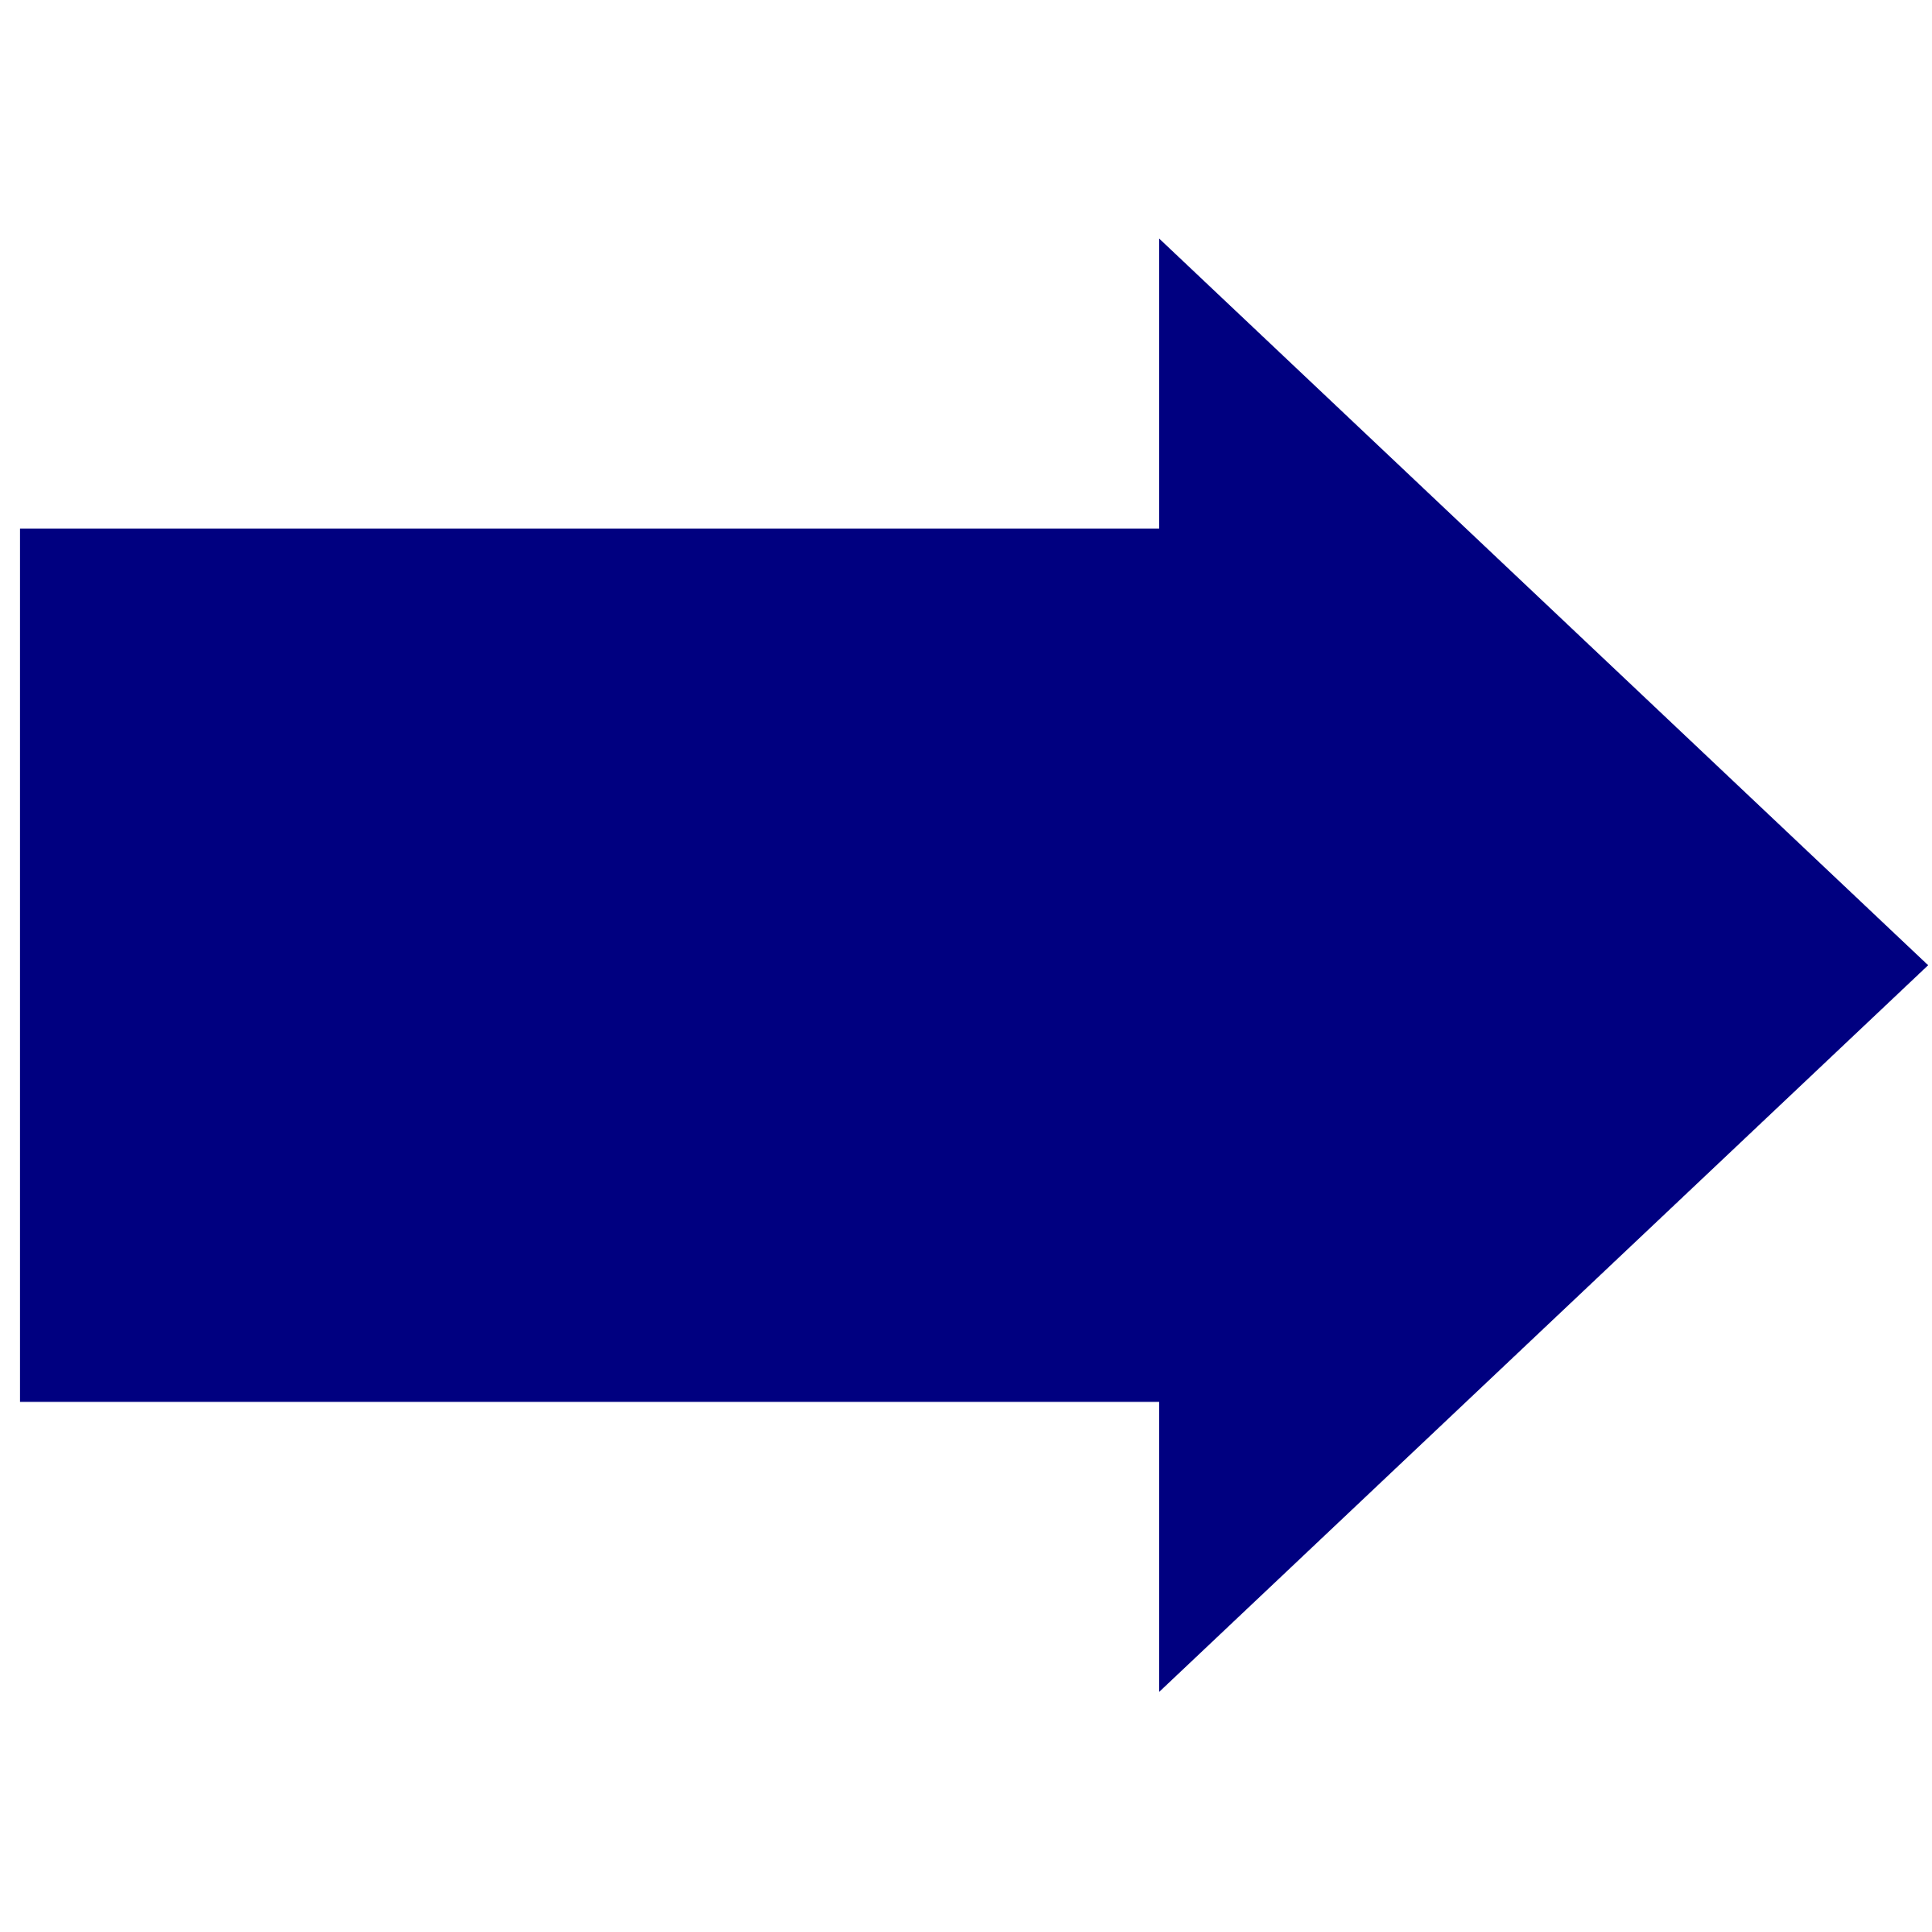
\includegraphics[width=0.8\linewidth]{BlueArrow}
%	\end{figure}
%\end{column}
\begin{column}{0.45\textwidth}
	\begin{figure} 	
 	
\includegraphics[width=0.2\linewidth,angle=45]{BlueArrowVertical}
 	 \end{figure}
 	 \vspace{-1.5em}
    \begin{block}{Security ${\color{red}\Rightarrow}$}
Preservation of $\simeq_{ctx}$
	\end{block}
\end{column}
\end{columns}
%Give some kind of intuition here (while speaking)!
}
\end{frame}
%------------------------------------------------
\begin{frame}
\frametitle{Proof: Correctness ${\color{red}\Leftarrow}$}
\begin{block}{Approach}
\begin{equation*}
\oldinference{
t\simeq_{ctx}t'\\
\compile{\vdash s}{t} & \compile{\vdash s'}{t'}\\
}{
s\simeq_{ctx}s'}
\end{equation*}
\center Techniques: compilation $[[\cdot]]$ + simulation relation $R$
\end{block}
\end{frame}

\begin{frame}
\frametitle{Proof: Correctness}
\vspace{-1em}
\begin{columns}
\begin{column}{0.65\textwidth}
\end{column}
\begin{column}{0.35\textwidth}
\begin{empheq}[box={\mybluebox[2pt][2pt]}]{flalign*}
\oldinference{
t\simeq_{ctx}t'\\
\compile{\vdash s}{t} & \compile{\vdash s'}{t'}\\
}{
s\simeq_{ctx}s'}
\end{empheq}
\end{column}

\end{columns}

\vspace{-1em}
%first & is for left alignment,third for middle and fifth for right
\begin{alignat*}{3}
&&{\color{red}{s}}\ &{\color{red}{\simeq^?_{ctx}s'}}&&\\
&&&\Updownarrow& \text{definition } \simeq_{ctx}&\\
 \forall C\ldotp\quad C[s&]\Downarrow\ &&{\color{red}{\Rightarrow^?}}  & C[s'&]\Downarrow \\
&\Downarrow coherence &&&&\Uparrow coherence\\
\vdash C[s&]\Downarrow\ && & \vdash C[s'&]\Downarrow \\
&\Downarrow {\color{mGreen}{*}} &&&&\Uparrow {\color{mGreen}{*}}\\
[[C]][t&]\Downarrow\ &&\Rightarrow & [[C]][t'&]\Downarrow \\
&&&\Updownarrow& \text{definition } \simeq_{ctx}&\\
&&{\color{mGreen}{t}}\ &{\color{mGreen}{\simeq_{ctx}t'}}&&\\
\end{alignat*}
\vspace{-3em}
\begin{equation*}
{\color{mGreen}{*}}\ \textbf{Lemma's: }\simrelcom{\vdash C[s]}{[[C]]{\color{mGreen}{[}}[[s]]{\color{mGreen}{]}}},\ \simrelcom{\vdash x}{y} \Rightarrow\ \vdash x \Downarrow\ \Leftrightarrow y \Downarrow 
\end{equation*}
\end{frame}
%------------------------------------------------
\begin{frame}
\frametitle{Proof: Security ${\color{red}\Rightarrow}$}
\begin{block}{Approach}
\begin{equation*}
\oldinference{
s\simeq_{ctx}s'\\ 
\compile{\vdash s}{t} & \compile{\vdash s'}{t'}\\
}{
t\simeq_{ctx}t'}
\end{equation*}
\center Techniques: back-translation $\backtranslation{\cdot}$ + simulation relation $R$
\end{block}
\end{frame}
%------------------------------------------------
\begin{frame}
\frametitle{Proof: Security}
\vspace{-1em}
\begin{columns}
\begin{column}{0.65\textwidth}
\end{column}
\begin{column}{0.35\textwidth}
\begin{empheq}[box={\mybluebox[2pt][2pt]}]{flalign*}
\oldinference{
s\simeq_{ctx}s'\\ 
\compile{\vdash s}{t} & \compile{\vdash s'}{t'}\\
}{
t\simeq_{ctx}t'}
\end{empheq}
\end{column}

\end{columns}

\vspace{-1em}
%first & is for left alignment,third for middle and fifth for right
\begin{alignat*}{3}
&&{\color{mGreen}{s}}\ &{\color{mGreen}{\simeq_{ctx}s'}}&&\\
&&&\Updownarrow& \text{definition } \simeq_{ctx}&\\
  \backtranslation{C}[s&]\Downarrow\ && \Rightarrow  & \backtranslation{C}[s'&]\Downarrow \\
&\Uparrow coherence &&&&\Downarrow coherence\\
\vdash \backtranslation{C}[s&]\Downarrow\ && & \vdash \backtranslation{C}[s'&]\Downarrow \\
&\Uparrow {\color{mGreen}{*}} &&&&\Downarrow {\color{mGreen}{*}}\\
\forall C\ldotp\quad C [t&]\Downarrow\ &&{\color{red}{\Rightarrow^?}} &  C[t'&]\Downarrow \\
&&&\Updownarrow& \text{definition } \simeq_{ctx}&\\
&&{\color{red}{t}}\ &{\color{red}{\simeq^?_{ctx}t'}}&&\\
\end{alignat*}
\vspace{-3em}
\begin{equation*}
{\color{mGreen}{*}}\ \textbf{Lemma's: }\simrelcom{(\vdash \backtranslation{C}[s])}{C{\color{mGreen}{[}}[[s]]{\color{mGreen}{]}}},\ \simrelcom{\vdash x}{y} \Rightarrow\ \vdash x \Downarrow\ \Leftrightarrow y \Downarrow 
\end{equation*}
\end{frame}

%------------------------------------------------

\begin{frame}[fragile]
\frametitle{Proof: Security - back-translation example}
\textbf{Intuition}:\\
\begin{itemize}
\item Construct minimal contract for context functions\\
\item Insert assertions where necessary\\
\item \textbf{Goal}: prove that $\vdash \backtranslation{C}[s] \Downarrow\ \Leftrightarrow C[t] \Downarrow $

\end{itemize}

\textbf{Example}:\\
\begin{columns}
\begin{column}{0.4\textwidth}

\begin{figure}[h]
  \centering
\begin{lstlisting}[style=CStyleNoNum, captionpos = t,title = Target]
int f(int* a, int b){
	free(a);
	b = 5; 
	return b;
}
\end{lstlisting}
\end{figure}
	
\end{column}

\begin{column}{0.08\textwidth}

	{\large$\backtranslation{\cdot}$}\\\vspace{-1em}
	\begin{figure}
	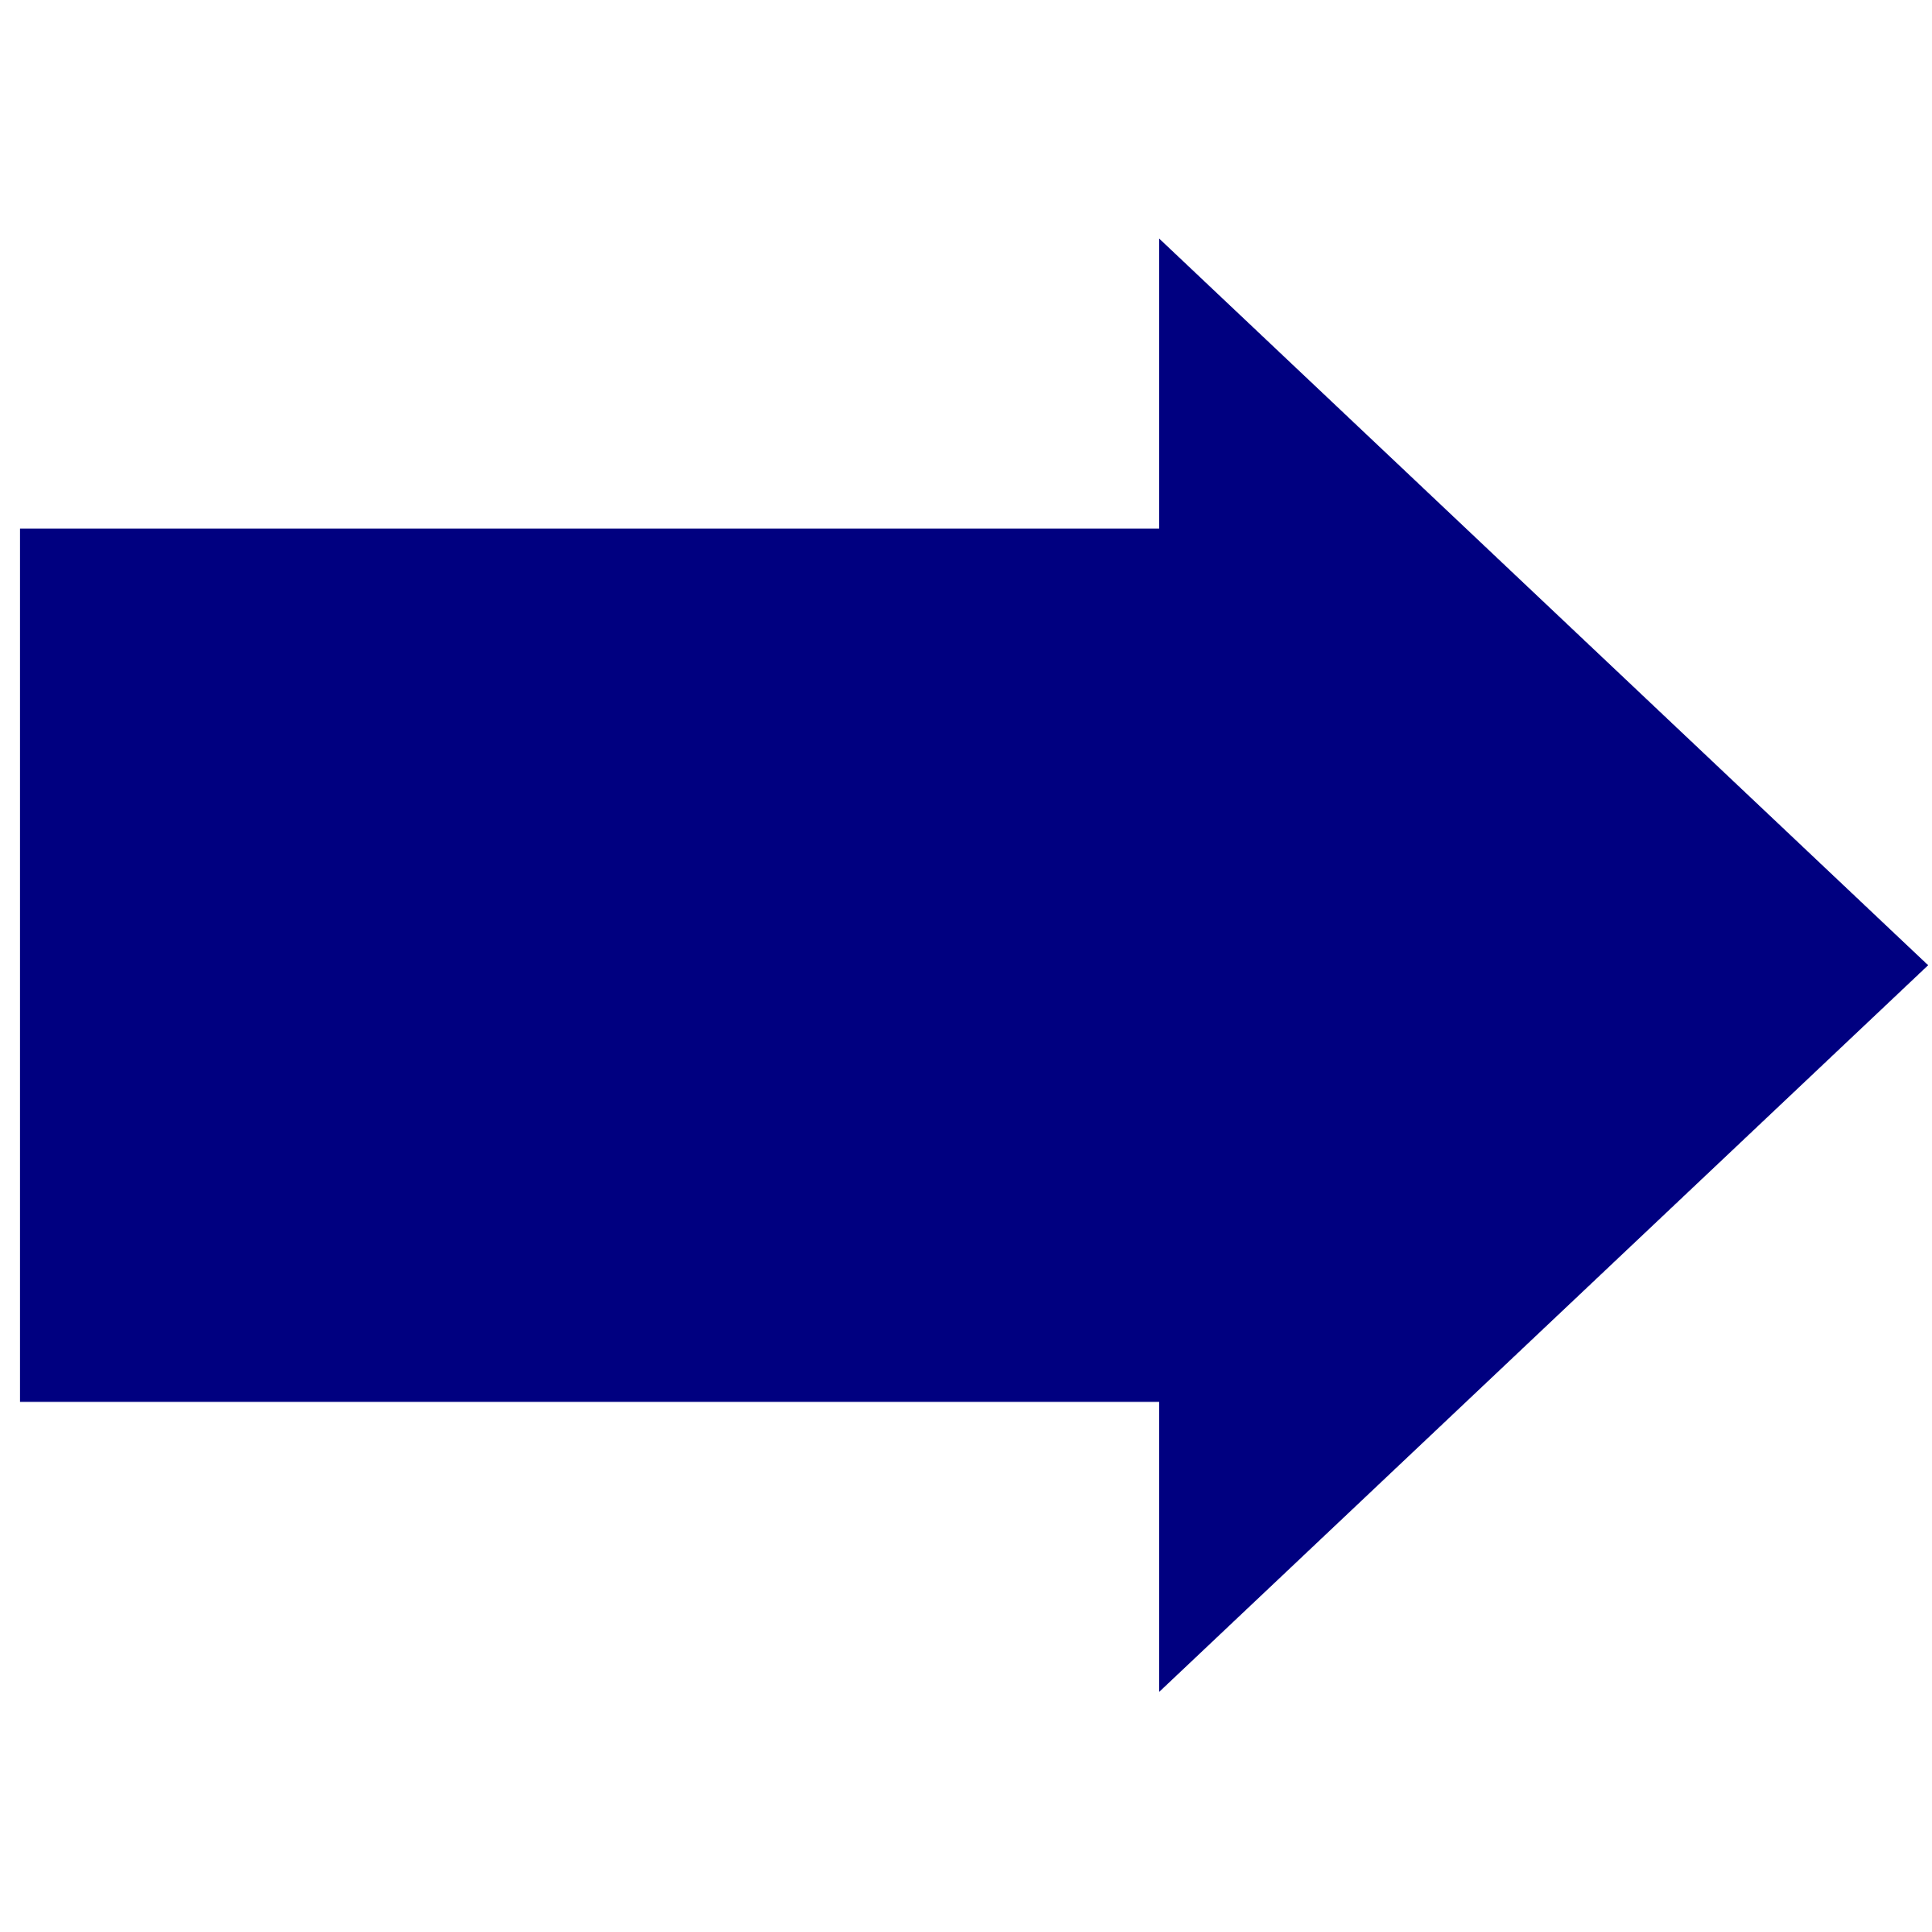
\includegraphics[width=0.8\linewidth]{BlueArrow}
	\end{figure}

\end{column}

\begin{column}{0.56\textwidth}

\begin{figure}[h]
  \centering
\begin{lstlisting}[style=CStyleNoNum, captionpos = t,title = Source]
int f(int* a, int b)
//@pre (a${\color{mGreen}{_{chunk}}}$: a |-> [_]${\color{mGreen}{_L) \lor a = null}}$;
//@post true;
{
	(...)
}
\end{lstlisting}
\end{figure}   

\end{column}
\end{columns}

\end{frame}
%------------------------------------------------
\begin{frame}[fragile]
\frametitle{Proof: Security - back-translation example}
\textbf{Intuition}:\\
\begin{itemize}
\item Construct minimal contract for context functions\\
\item Insert assertions where necessary\\
\end{itemize}

\textbf{Example}:\\
\begin{columns}
\begin{column}{0.4\textwidth}

\begin{figure}[h]
  \centering
\begin{lstlisting}[style=CStyleNoNum, captionpos = t,title = Target]
int f(int* a, int b){
	free(a);
	(...)
}
\end{lstlisting}
\end{figure}
	
\end{column}

\begin{column}{0.08\textwidth}

	{\large$\backtranslation{\cdot}$}\\\vspace{-1em}
	\begin{figure}
	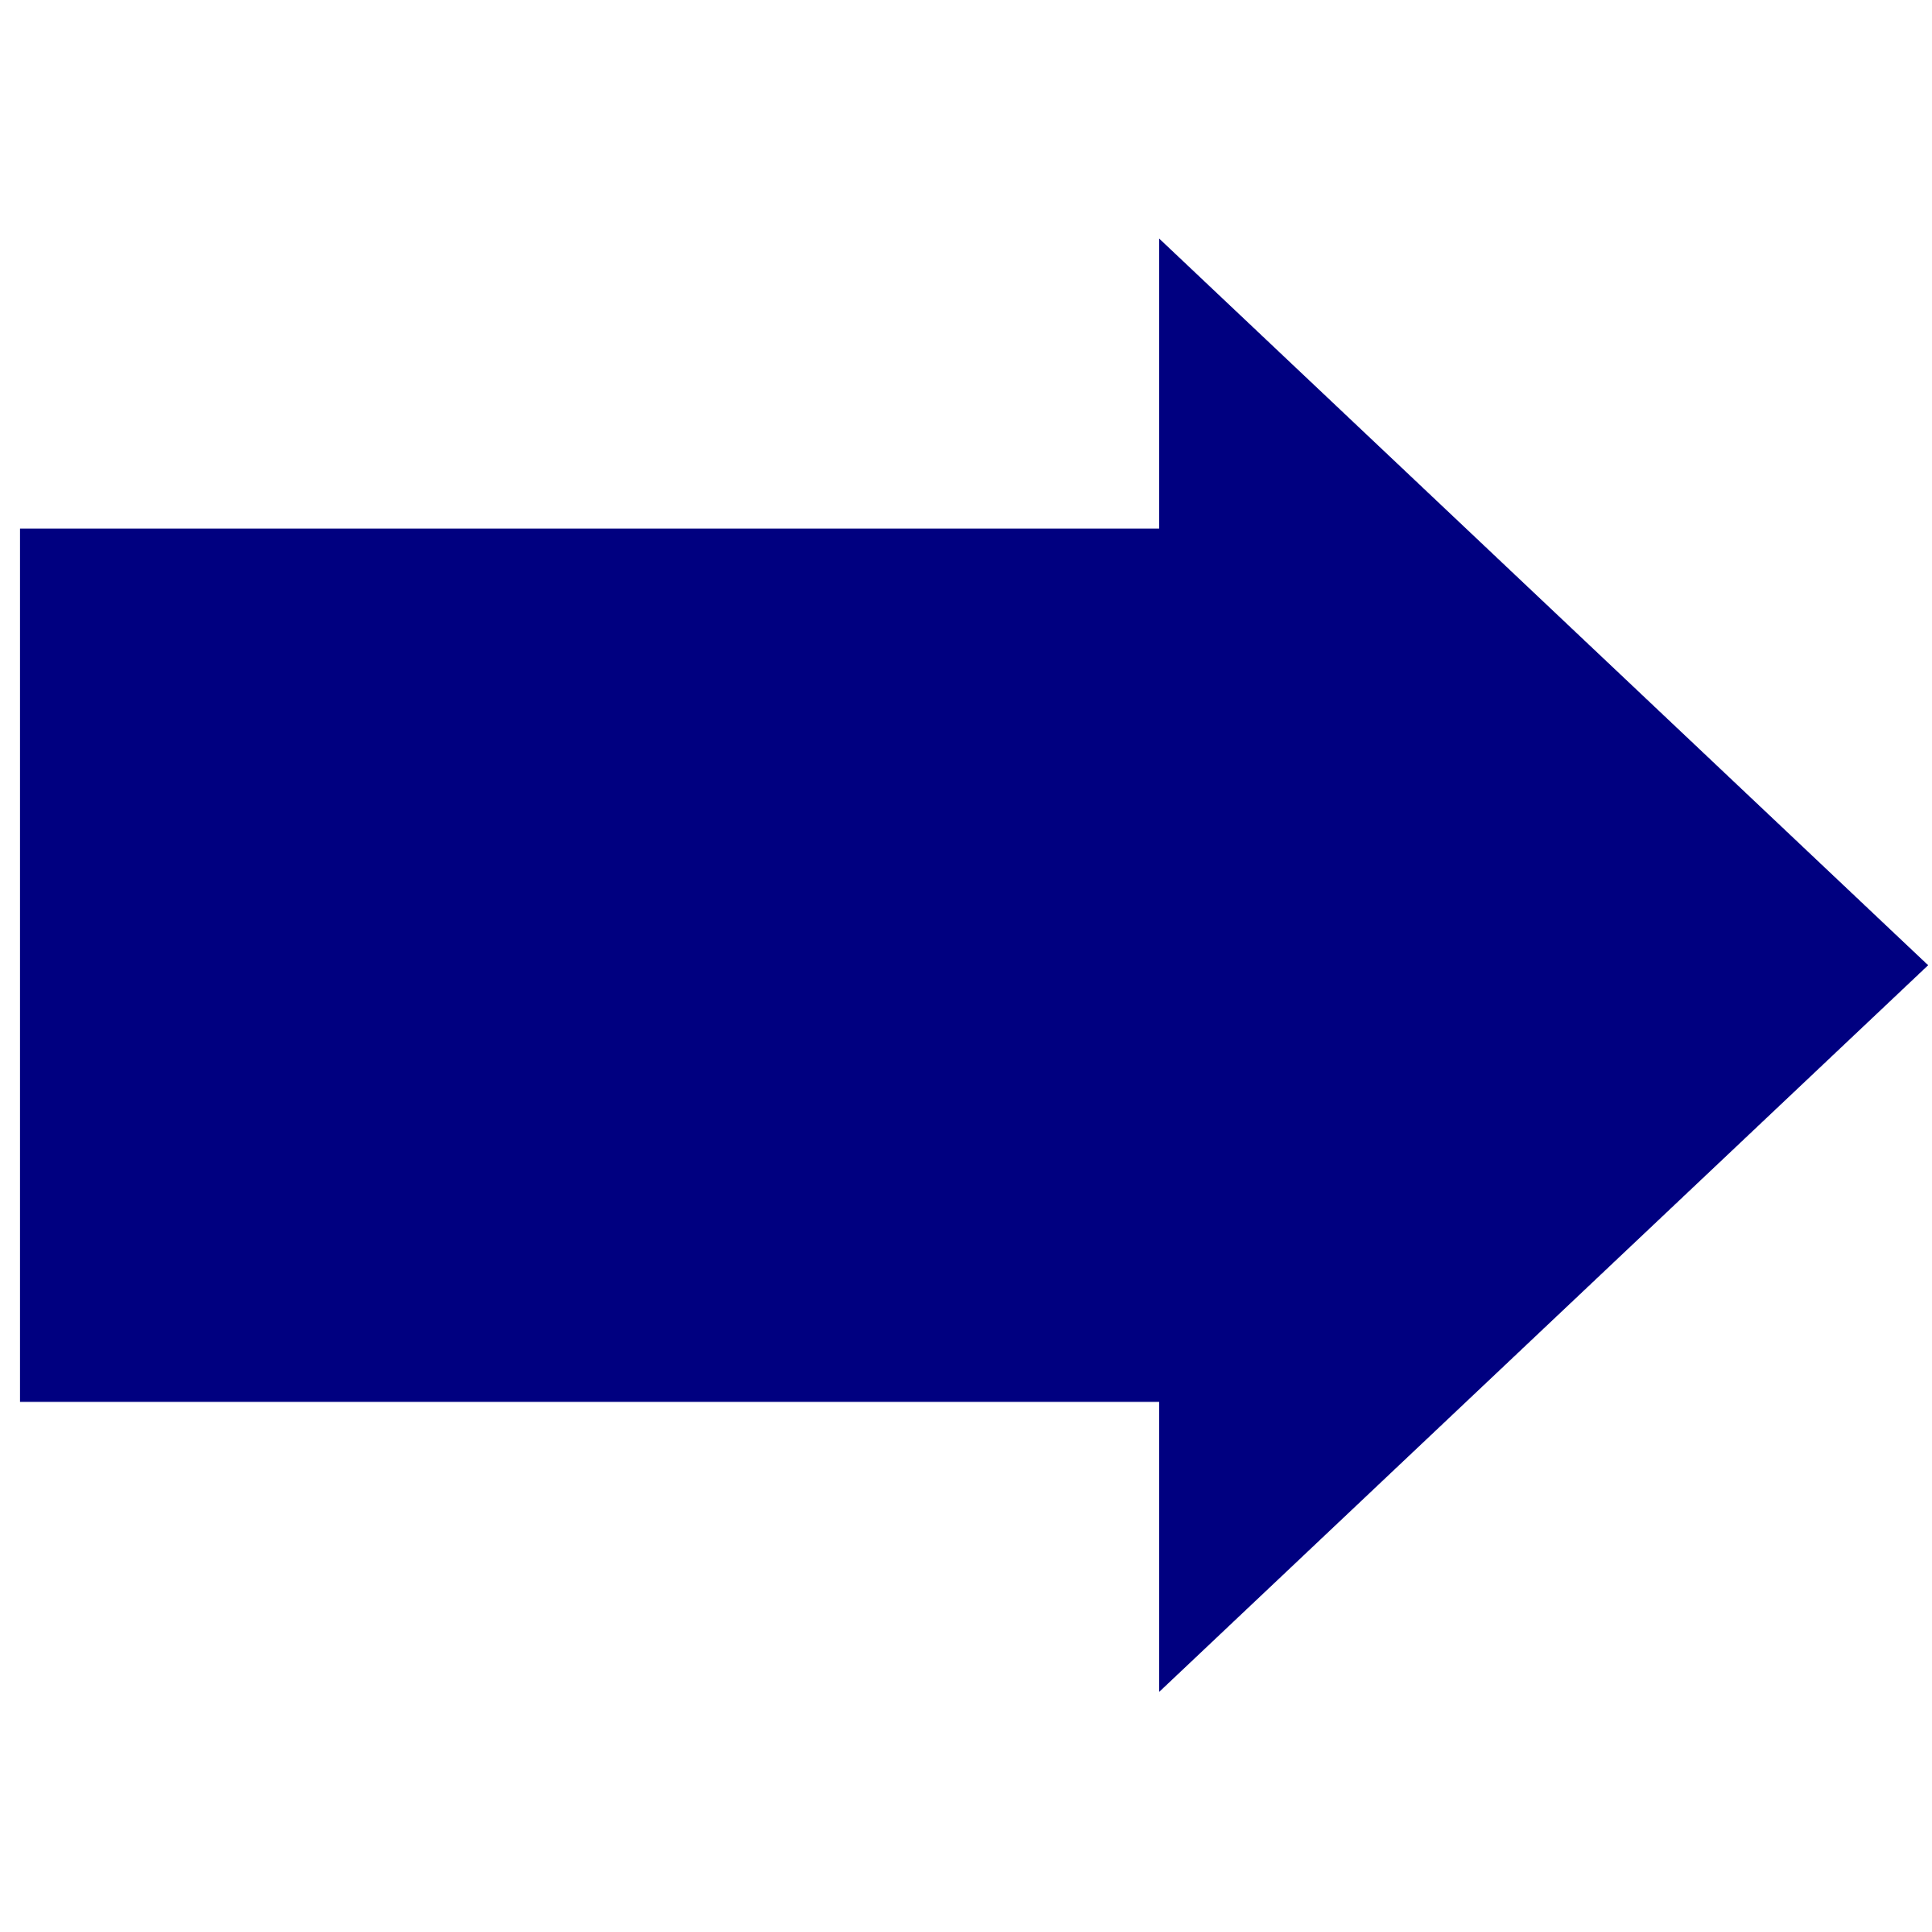
\includegraphics[width=0.8\linewidth]{BlueArrow}
	\end{figure}

\end{column}

\begin{column}{0.56\textwidth}

\begin{figure}[h]
  \centering
\begin{lstlisting}[style=CStyleNoNum, captionpos = t,title = Source]
int f(int* a, int b)
//@pre (a${\color{mGreen}{_{chunk}}}$: a |-> [_]${\color{mGreen}{_L) \lor a = null}}$;
//@post true;
{
	//{(a${\color{mGreen}{_{chunk}}}$: a |-> [_]${\color{mGreen}{_L) \lor a = null}}$}
	assert(a != null);
	//{a${\color{mGreen}{_{chunk}}}$: a |-> [_]${\color{mGreen}{_L}}$}
	free(a);
	//{}
	(...)
}
\end{lstlisting}
\end{figure}   

\end{column}
\end{columns}

\end{frame}
%------------------------------------------------

\begin{frame}[fragile]
\frametitle{Proof: Security - back-translation example}
\textbf{Intuition}:\\
\begin{itemize}
\item Construct minimal contract for context functions\\
\item Insert assertions where necessary\\
\end{itemize}

\textbf{Example}:\\
\begin{columns}
\begin{column}{0.4\textwidth}

\begin{figure}[h]
  \centering
\begin{lstlisting}[style=CStyleNoNum, captionpos = t,title = Target]
int f(int* a, int b){
	(...)
	b = 5; 
	return b;
}
\end{lstlisting}
\end{figure}
	
\end{column}

\begin{column}{0.08\textwidth}

	{\large$\backtranslation{\cdot}$}\\\vspace{-1em}
	\begin{figure}
	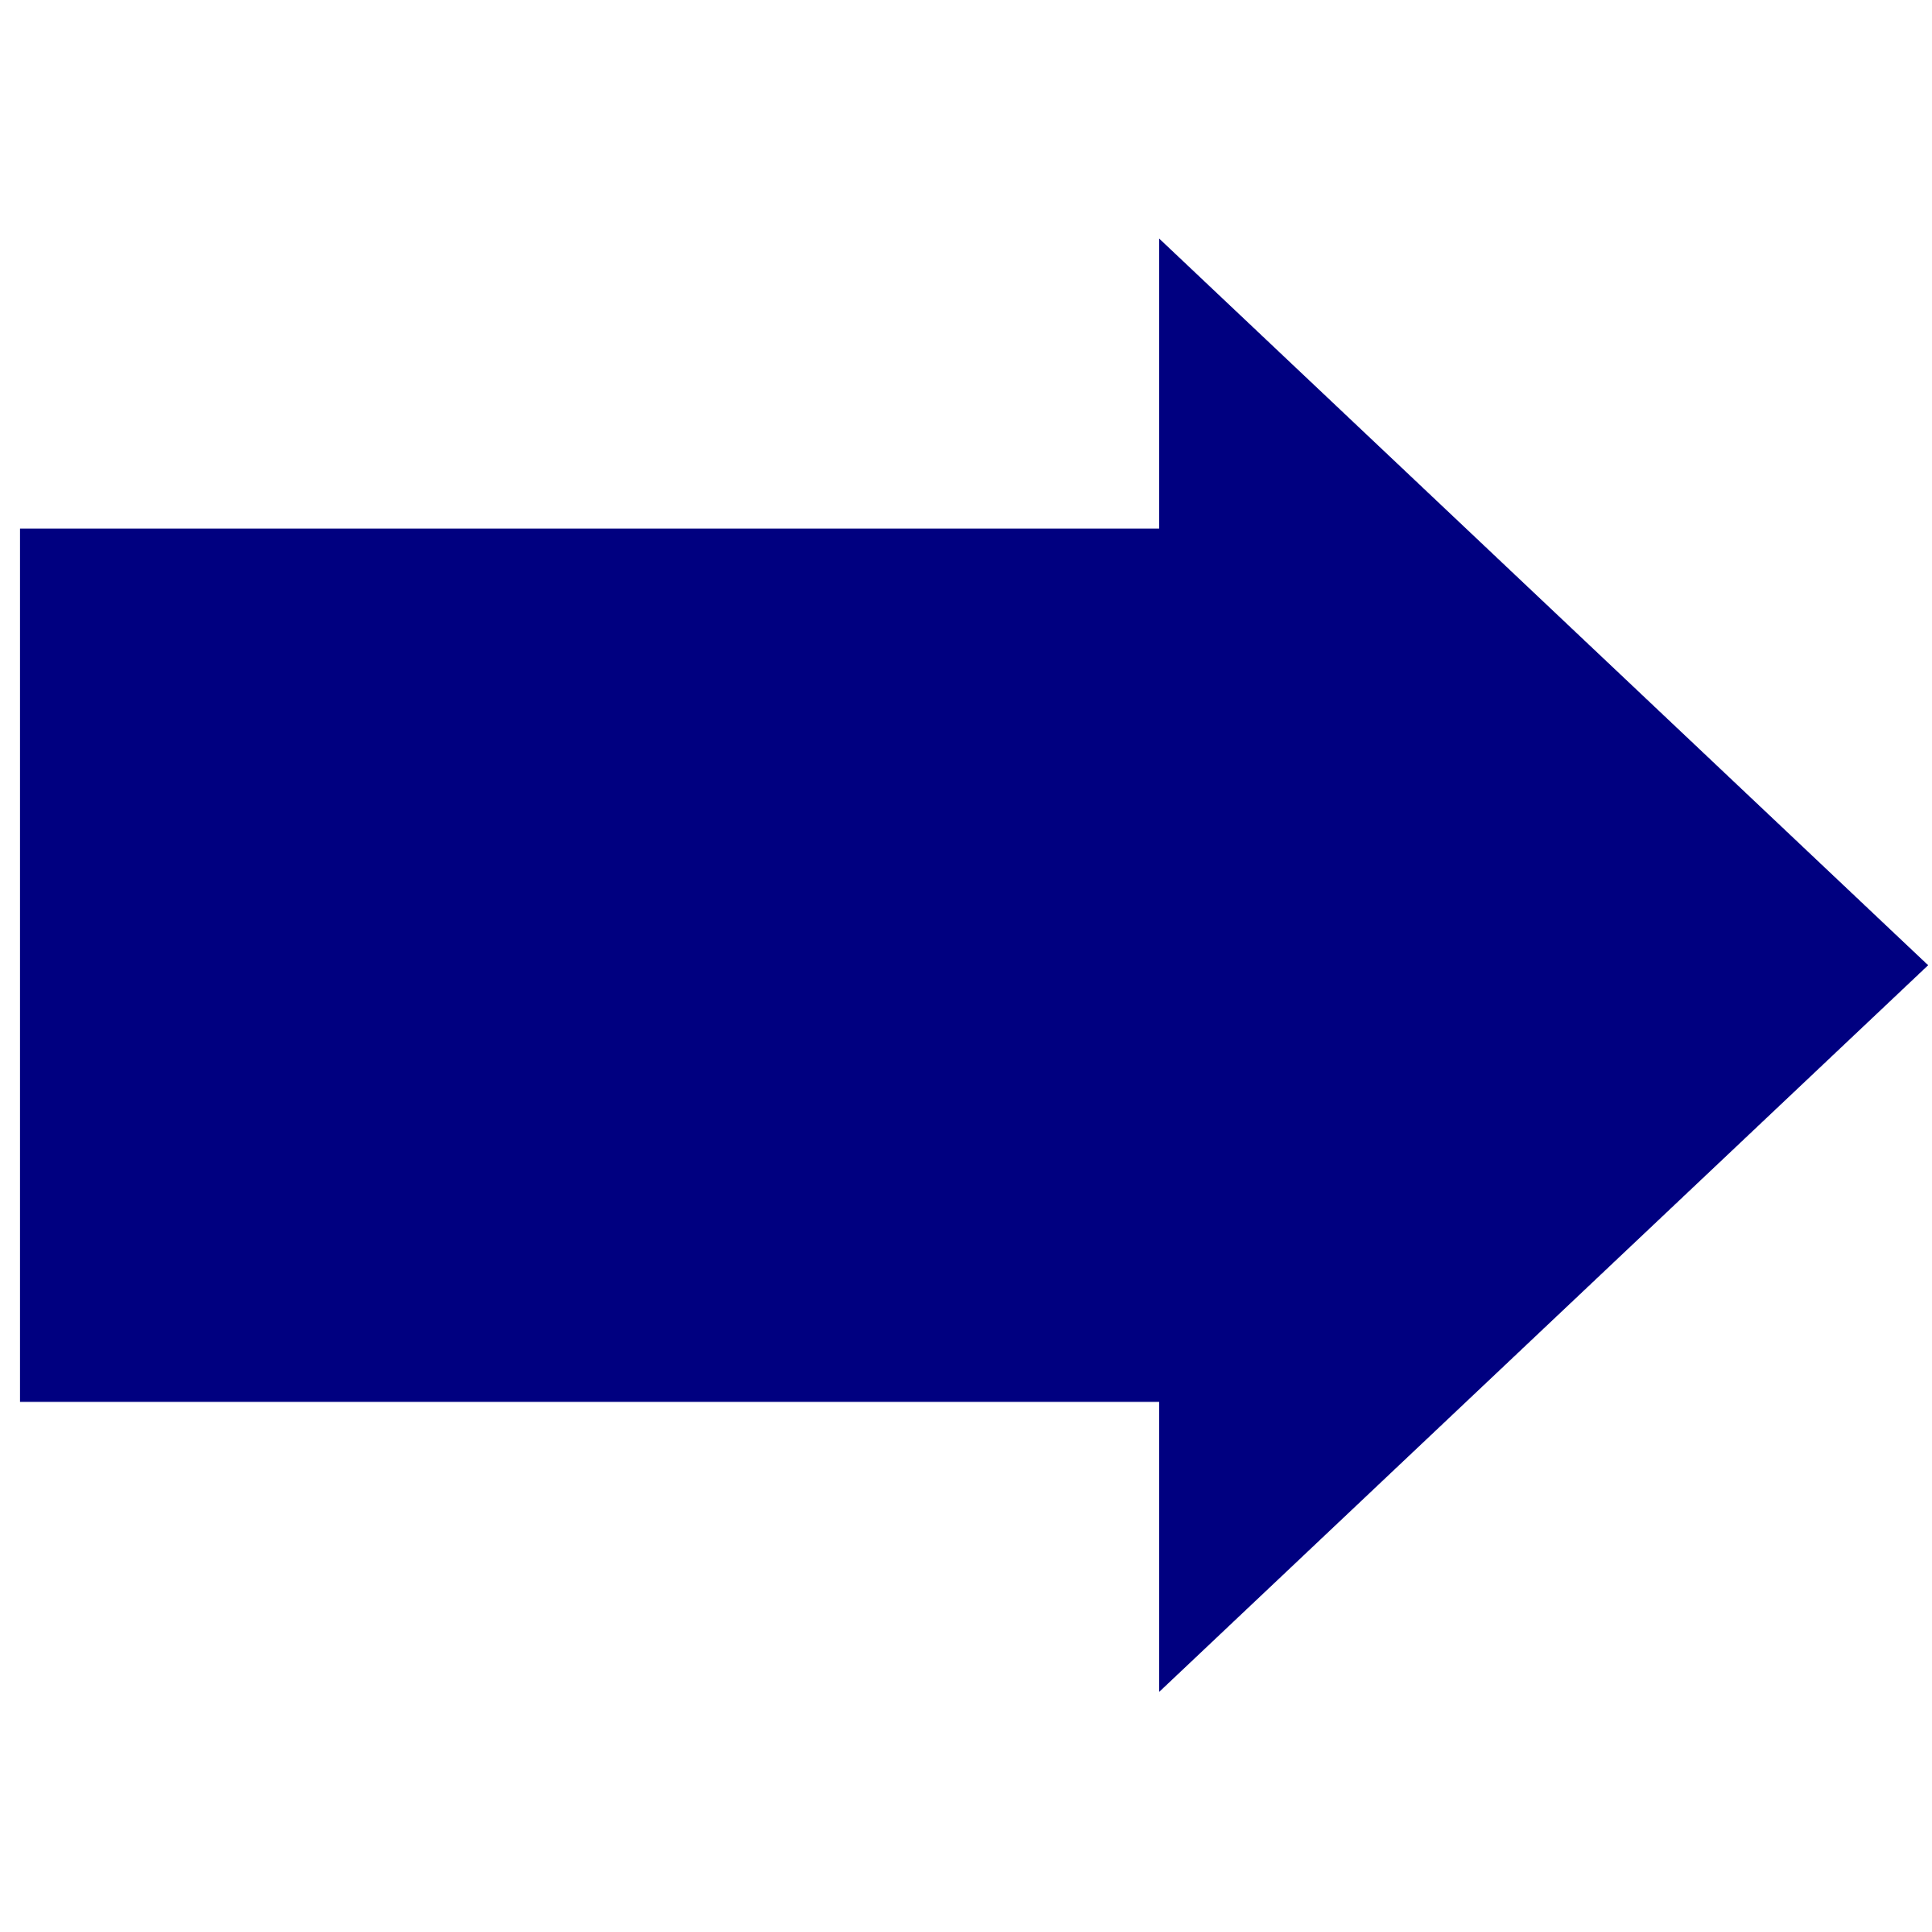
\includegraphics[width=0.8\linewidth]{BlueArrow}
	\end{figure}

\end{column}

\begin{column}{0.56\textwidth}

\begin{figure}[h]
  \centering
\begin{lstlisting}[style=CStyleNoNum, captionpos = t,title = Source]
int f(int* a, int b)
//@pre (a${\color{mGreen}{_{chunk}}}$: a |-> [_]${\color{mGreen}{_L) \lor a = null}}$;
//@post true;
{
	(...)
	//{}
	b = 5;
	//{b = 5} 
	return b;
	//{result = 5 * b = 5}
	//{}
}
\end{lstlisting}
\end{figure}   

\end{column}
\end{columns}

\end{frame}
\fi
%------------------------------------------------
\section{Conclusion and progress}

\begin{frame}
\frametitle{Conclusion and progress}
\begin{itemize}
\item Compiler from verified C to unverified C with (linear) capabilities 
\item \textbf{Claim}: Full Abstraction\\
%\qquad$\Rightarrow$ Gave some proof intuition
\item \textbf{State}: \\
\qquad $\sim$ Proven\\
  \qquad\qquad Technical report is lacking some details\\
 \qquad Currently writing submission for POPL\\
\end{itemize}
\end{frame}

%------------------------------------------------
\section{ADS progress report}

\begin{frame}
\frametitle{ADS progress}
\begin{itemize}
\item Publications:
	\begin{itemize}
	\item Thomas Van Strydonck, Dominique Devriese, Frank Piessens. Linear capabilities for modular fully-abstract compilation of verified code. Peer reviewed extended abstract. Talk at \emph{PRISC 2018}  (Principles of Secure Compilation; a workshop at the ACM-supported \emph{POPL} conference), January 2018.
	\item POPL 2019 submission currently being written (due 12 July 2018): Thomas Van Strydonck, Dominique Devriese, Frank Piessens. Linear capabilities for fully abstract compilation of separation-logic-verified code.
	\end{itemize}
\item The formal course units to be followed during the doctoral training programme:
	\begin{itemize}
	\item OPLSS summer school (4sp)
	\item Intensive academic writing course (SET) (2sp)	
	\end{itemize}
\end{itemize}
\end{frame}

\begin{frame}
\frametitle{ADS progress}
\begin{itemize}
\item Current contribution to bachelor and master education (work decided on yearly basis)
	\begin{itemize}
	\item Submitted thesis proposal for 2018-2019 (\emph{Developing attestation for capability machines})
	\item Taught \emph{Modelling of Complex Systems}  exercise sessions
	\item Supervised \emph{Probleemoplossen en ontwerpen, deel 3} exercise sessions and evaluated students
	\item Supervised a \emph{Software-ontwerp} project group and aided in oral examination
	\item Corrected exams for \emph{Methodiek van de informatica}
	\item Exam supervision each semester
	\end{itemize}
\end{itemize}
\end{frame}

\begin{frame}
\frametitle{ADS progress}
\vspace{-.5em}
\begin{itemize}
\item A detailed research plan of the doctoral project:
	\begin{itemize}
	\item WP1: Fully abstract compilation of verified C (Today's presentation)
	\item WP2: Extending WP1 to more realistic settings (A: Compiling non-annotated code, B: cooperating with non-compliant code)
	\item WP3: Fully abstract compilation of Rust
	\end{itemize}
\end{itemize}



\begin{figure}[ht]
\hspace*{-1cm}
\scalebox{.5}{
\makebox[\textwidth][c]{
     \begin{ganttchart}[%Specs
     x unit=0.25cm,
     y unit title=0.5cm,
     y unit chart=0.7cm,
     vgrid = {*{10}{gray!40!white,, line width={5mm}},{gray!40!white,, line width={5mm}},{thick,black},*{2}{dashed,gray},gray,*{2}{dashed,gray},gray,*{2}{dashed,gray},gray,*{2}{dashed,gray},{thick,black},*{2}{dashed,gray},gray,*{2}{dashed,gray},gray,*{2}{dashed,gray},gray,*{2}{dashed,gray},{thick,black},*{2}{dashed,gray},gray,*{2}{dashed,gray},gray,*{2}{dashed,gray},gray,*{2}{dashed,gray},{thick,black},*{2}{dashed,gray},gray,*{2}{dashed,gray},gray,*{2}{dashed,gray},gray,*{2}{dashed,gray},{thick,black},},
     %hgrid,
     title height=1,
%     title/.style={fill=none},
     title label font=\bfseries\footnotesize,
     bar/.style={fill=blue},
     bar height=0.7,
%   progress label text={},
     group right shift=0,
     group top shift=0.3,%0.7,
     %group bottom shift=0.3,%0.7,
     group height=.3,
     group peaks width={1},]{1}{60}
    %labels
    \ganttset{title/.append style={fill=gray!40!white}}
    \gantttitle[]{Y0}{12}
    \ganttset{title/.append style={fill=white}}
 
    \gantttitle[]{Y1}{12}                 % title 2
    \gantttitle[]{Y2}{12}
    \gantttitle[]{Y3}{12}                 % title 2
    \gantttitle[]{Y4}{12} \\              
	
    \ganttset{title/.append style={fill=gray!40!white}}	
	\gantttitle{Q1}{3}                      % title 3
    \gantttitle{Q2}{3}
    \gantttitle{Q3}{3}
    \gantttitle{Q4}{3}
    \ganttset{title/.append style={fill=white}}
	
	\gantttitle{Q1}{3}                      % title 3
    \gantttitle{Q2}{3}
    \gantttitle{Q3}{3}
    \gantttitle{Q4}{3}
    \gantttitle{Q1}{3}
    \gantttitle{Q2}{3}
    \gantttitle{Q3}{3} 
    \gantttitle{Q4}{3}    
    \gantttitle{Q1}{3}                      % title 3
    \gantttitle{Q2}{3}
    \gantttitle{Q3}{3}
    \gantttitle{Q4}{3}
    \gantttitle{Q1}{3}
    \gantttitle{Q2}{3}
    \gantttitle{Q3}{3} 
    \gantttitle{Q4}{3}\\
    
    % Setting group if any
     \ganttset{
       bar/.append style={draw=black,fill=green!40},
       group/.append style={draw=black, fill=green!40},} %
    \ganttgroup{WP1}{1}{42}\\ 
    \ganttbar{Research}{1}{21}\\
    \ganttbar[bar/.append style={top color=green!40, bottom color=red!40}]{Bundling}{37}{42}\ganttnewline[black]

     \ganttset{
       bar/.append style={draw=black,fill=red!40},
       group/.append style={draw=black, fill=red!40},}
    \ganttgroup{WP2}{19}{42} \\ 
    \ganttbar{Research WP2A}{19}{30} \\
    \ganttbar{Research WP2B}{28}{36} \\
    \ganttbar[bar/.append style={top color=green!40, bottom color=red!40}]{Bundling}{37}{42}\ganttnewline[black]
    
    \ganttset{
       bar/.append style={draw=black,fill=blue!40},
       group/.append style={draw=black, fill=blue!40},}
    \ganttgroup{WP3}{34}{60} \\ 
    \ganttbar{Research}{34}{54} \ganttnewline[black]

    \ganttset{
       bar/.append style={draw=black,fill=gray!40},
       group/.append style={draw=black, fill=gray!40},}
    \ganttgroup{Reporting}{20}{60} \\ 
    
    \ganttbar{Conference publ.}{20}{21} 
    \ganttbar[inline=true, name = c1,bar inline label node/.style={above=0.3pt,font=\bfseries},bar/.append style={fill=green!40}]{C1}{20}{21} 
	\ganttbar[inline=true, name = c2,bar inline label node/.style={above=0.3pt,font=\bfseries},bar/.append style={fill=red!40}]{C2}{35}{36}
	\ganttbar[inline=true, name = c3,bar inline label node/.style={above=0.3pt,font=\bfseries},bar/.append style={fill=blue!40}]{C3}{53}{54}\\
	 
    \ganttbar{Journal publ.}{41}{42} 
    \ganttbar[inline=true, name = j1,bar inline label node/.style={above=0.3pt,font=\bfseries},bar/.append style={top color=green!40, bottom color=red!40}]{J1}{41}{42} 
	\ganttbar[inline=true, name = j2,bar inline label node/.style={above=0.3pt,font=\bfseries},bar/.append style={fill=blue!40}]{J2}{59}{60}\\
	 
	\ganttbar{Thesis text}{55}{60} %\\ 

\end{ganttchart}
}
}
%    \caption{Proposed planning of the PhD project}
    \label{gchart}
\end{figure}
\end{frame}

\end{document}
